% Options for packages loaded elsewhere
% Options for packages loaded elsewhere
\PassOptionsToPackage{unicode}{hyperref}
\PassOptionsToPackage{hyphens}{url}
\PassOptionsToPackage{dvipsnames,svgnames,x11names}{xcolor}
%
\documentclass[
]{article}
\usepackage{xcolor}
\usepackage{amsmath,amssymb}
\setcounter{secnumdepth}{5}
\usepackage{iftex}
\ifPDFTeX
  \usepackage[T1]{fontenc}
  \usepackage[utf8]{inputenc}
  \usepackage{textcomp} % provide euro and other symbols
\else % if luatex or xetex
  \usepackage{unicode-math} % this also loads fontspec
  \defaultfontfeatures{Scale=MatchLowercase}
  \defaultfontfeatures[\rmfamily]{Ligatures=TeX,Scale=1}
\fi
\usepackage{lmodern}
\ifPDFTeX\else
  % xetex/luatex font selection
\fi
% Use upquote if available, for straight quotes in verbatim environments
\IfFileExists{upquote.sty}{\usepackage{upquote}}{}
\IfFileExists{microtype.sty}{% use microtype if available
  \usepackage[]{microtype}
  \UseMicrotypeSet[protrusion]{basicmath} % disable protrusion for tt fonts
}{}
\makeatletter
\@ifundefined{KOMAClassName}{% if non-KOMA class
  \IfFileExists{parskip.sty}{%
    \usepackage{parskip}
  }{% else
    \setlength{\parindent}{0pt}
    \setlength{\parskip}{6pt plus 2pt minus 1pt}}
}{% if KOMA class
  \KOMAoptions{parskip=half}}
\makeatother
% Make \paragraph and \subparagraph free-standing
\makeatletter
\ifx\paragraph\undefined\else
  \let\oldparagraph\paragraph
  \renewcommand{\paragraph}{
    \@ifstar
      \xxxParagraphStar
      \xxxParagraphNoStar
  }
  \newcommand{\xxxParagraphStar}[1]{\oldparagraph*{#1}\mbox{}}
  \newcommand{\xxxParagraphNoStar}[1]{\oldparagraph{#1}\mbox{}}
\fi
\ifx\subparagraph\undefined\else
  \let\oldsubparagraph\subparagraph
  \renewcommand{\subparagraph}{
    \@ifstar
      \xxxSubParagraphStar
      \xxxSubParagraphNoStar
  }
  \newcommand{\xxxSubParagraphStar}[1]{\oldsubparagraph*{#1}\mbox{}}
  \newcommand{\xxxSubParagraphNoStar}[1]{\oldsubparagraph{#1}\mbox{}}
\fi
\makeatother

\usepackage{color}
\usepackage{fancyvrb}
\newcommand{\VerbBar}{|}
\newcommand{\VERB}{\Verb[commandchars=\\\{\}]}
\DefineVerbatimEnvironment{Highlighting}{Verbatim}{commandchars=\\\{\}}
% Add ',fontsize=\small' for more characters per line
\usepackage{framed}
\definecolor{shadecolor}{RGB}{241,243,245}
\newenvironment{Shaded}{\begin{snugshade}}{\end{snugshade}}
\newcommand{\AlertTok}[1]{\textcolor[rgb]{0.68,0.00,0.00}{#1}}
\newcommand{\AnnotationTok}[1]{\textcolor[rgb]{0.37,0.37,0.37}{#1}}
\newcommand{\AttributeTok}[1]{\textcolor[rgb]{0.40,0.45,0.13}{#1}}
\newcommand{\BaseNTok}[1]{\textcolor[rgb]{0.68,0.00,0.00}{#1}}
\newcommand{\BuiltInTok}[1]{\textcolor[rgb]{0.00,0.23,0.31}{#1}}
\newcommand{\CharTok}[1]{\textcolor[rgb]{0.13,0.47,0.30}{#1}}
\newcommand{\CommentTok}[1]{\textcolor[rgb]{0.37,0.37,0.37}{#1}}
\newcommand{\CommentVarTok}[1]{\textcolor[rgb]{0.37,0.37,0.37}{\textit{#1}}}
\newcommand{\ConstantTok}[1]{\textcolor[rgb]{0.56,0.35,0.01}{#1}}
\newcommand{\ControlFlowTok}[1]{\textcolor[rgb]{0.00,0.23,0.31}{\textbf{#1}}}
\newcommand{\DataTypeTok}[1]{\textcolor[rgb]{0.68,0.00,0.00}{#1}}
\newcommand{\DecValTok}[1]{\textcolor[rgb]{0.68,0.00,0.00}{#1}}
\newcommand{\DocumentationTok}[1]{\textcolor[rgb]{0.37,0.37,0.37}{\textit{#1}}}
\newcommand{\ErrorTok}[1]{\textcolor[rgb]{0.68,0.00,0.00}{#1}}
\newcommand{\ExtensionTok}[1]{\textcolor[rgb]{0.00,0.23,0.31}{#1}}
\newcommand{\FloatTok}[1]{\textcolor[rgb]{0.68,0.00,0.00}{#1}}
\newcommand{\FunctionTok}[1]{\textcolor[rgb]{0.28,0.35,0.67}{#1}}
\newcommand{\ImportTok}[1]{\textcolor[rgb]{0.00,0.46,0.62}{#1}}
\newcommand{\InformationTok}[1]{\textcolor[rgb]{0.37,0.37,0.37}{#1}}
\newcommand{\KeywordTok}[1]{\textcolor[rgb]{0.00,0.23,0.31}{\textbf{#1}}}
\newcommand{\NormalTok}[1]{\textcolor[rgb]{0.00,0.23,0.31}{#1}}
\newcommand{\OperatorTok}[1]{\textcolor[rgb]{0.37,0.37,0.37}{#1}}
\newcommand{\OtherTok}[1]{\textcolor[rgb]{0.00,0.23,0.31}{#1}}
\newcommand{\PreprocessorTok}[1]{\textcolor[rgb]{0.68,0.00,0.00}{#1}}
\newcommand{\RegionMarkerTok}[1]{\textcolor[rgb]{0.00,0.23,0.31}{#1}}
\newcommand{\SpecialCharTok}[1]{\textcolor[rgb]{0.37,0.37,0.37}{#1}}
\newcommand{\SpecialStringTok}[1]{\textcolor[rgb]{0.13,0.47,0.30}{#1}}
\newcommand{\StringTok}[1]{\textcolor[rgb]{0.13,0.47,0.30}{#1}}
\newcommand{\VariableTok}[1]{\textcolor[rgb]{0.07,0.07,0.07}{#1}}
\newcommand{\VerbatimStringTok}[1]{\textcolor[rgb]{0.13,0.47,0.30}{#1}}
\newcommand{\WarningTok}[1]{\textcolor[rgb]{0.37,0.37,0.37}{\textit{#1}}}

\usepackage{longtable,booktabs,array}
\newcounter{none} % for unnumbered tables
\usepackage{calc} % for calculating minipage widths
% Correct order of tables after \paragraph or \subparagraph
\usepackage{etoolbox}
\makeatletter
\patchcmd\longtable{\par}{\if@noskipsec\mbox{}\fi\par}{}{}
\makeatother
% Allow footnotes in longtable head/foot
\IfFileExists{footnotehyper.sty}{\usepackage{footnotehyper}}{\usepackage{footnote}}
\makesavenoteenv{longtable}
\usepackage{graphicx}
\makeatletter
\newsavebox\pandoc@box
\newcommand*\pandocbounded[1]{% scales image to fit in text height/width
  \sbox\pandoc@box{#1}%
  \Gscale@div\@tempa{\textheight}{\dimexpr\ht\pandoc@box+\dp\pandoc@box\relax}%
  \Gscale@div\@tempb{\linewidth}{\wd\pandoc@box}%
  \ifdim\@tempb\p@<\@tempa\p@\let\@tempa\@tempb\fi% select the smaller of both
  \ifdim\@tempa\p@<\p@\scalebox{\@tempa}{\usebox\pandoc@box}%
  \else\usebox{\pandoc@box}%
  \fi%
}
% Set default figure placement to htbp
\def\fps@figure{htbp}
\makeatother


% definitions for citeproc citations
\NewDocumentCommand\citeproctext{}{}
\NewDocumentCommand\citeproc{mm}{%
  \begingroup\def\citeproctext{#2}\cite{#1}\endgroup}
\makeatletter
 % allow citations to break across lines
 \let\@cite@ofmt\@firstofone
 % avoid brackets around text for \cite:
 \def\@biblabel#1{}
 \def\@cite#1#2{{#1\if@tempswa , #2\fi}}
\makeatother
\newlength{\cslhangindent}
\setlength{\cslhangindent}{1.5em}
\newlength{\csllabelwidth}
\setlength{\csllabelwidth}{3em}
\newenvironment{CSLReferences}[2] % #1 hanging-indent, #2 entry-spacing
 {\begin{list}{}{%
  \setlength{\itemindent}{0pt}
  \setlength{\leftmargin}{0pt}
  \setlength{\parsep}{0pt}
  % turn on hanging indent if param 1 is 1
  \ifodd #1
   \setlength{\leftmargin}{\cslhangindent}
   \setlength{\itemindent}{-1\cslhangindent}
  \fi
  % set entry spacing
  \setlength{\itemsep}{#2\baselineskip}}}
 {\end{list}}
\usepackage{calc}
\newcommand{\CSLBlock}[1]{\hfill\break\parbox[t]{\linewidth}{\strut\ignorespaces#1\strut}}
\newcommand{\CSLLeftMargin}[1]{\parbox[t]{\csllabelwidth}{\strut#1\strut}}
\newcommand{\CSLRightInline}[1]{\parbox[t]{\linewidth - \csllabelwidth}{\strut#1\strut}}
\newcommand{\CSLIndent}[1]{\hspace{\cslhangindent}#1}



\setlength{\emergencystretch}{3em} % prevent overfull lines

\providecommand{\tightlist}{%
  \setlength{\itemsep}{0pt}\setlength{\parskip}{0pt}}



 


\usepackage{booktabs}
\usepackage{longtable}
\usepackage{array}
\usepackage{multirow}
\usepackage{wrapfig}
\usepackage{float}
\usepackage{colortbl}
\usepackage{pdflscape}
\usepackage{tabu}
\usepackage{threeparttable}
\usepackage{threeparttablex}
\usepackage[normalem]{ulem}
\usepackage{makecell}
\usepackage{xcolor}
\usepackage{float}
\usepackage{etoolbox}
\pretocmd{\tableofcontents}{\clearpage}{}{}
\apptocmd{\tableofcontents}{\clearpage}{}{}
\usepackage{geometry}
\geometry{margin=1in}
\makeatletter
\@ifpackageloaded{caption}{}{\usepackage{caption}}
\AtBeginDocument{%
\ifdefined\contentsname
  \renewcommand*\contentsname{Table of contents}
\else
  \newcommand\contentsname{Table of contents}
\fi
\ifdefined\listfigurename
  \renewcommand*\listfigurename{List of Figures}
\else
  \newcommand\listfigurename{List of Figures}
\fi
\ifdefined\listtablename
  \renewcommand*\listtablename{List of Tables}
\else
  \newcommand\listtablename{List of Tables}
\fi
\ifdefined\figurename
  \renewcommand*\figurename{Figure}
\else
  \newcommand\figurename{Figure}
\fi
\ifdefined\tablename
  \renewcommand*\tablename{Table}
\else
  \newcommand\tablename{Table}
\fi
}
\@ifpackageloaded{float}{}{\usepackage{float}}
\floatstyle{ruled}
\@ifundefined{c@chapter}{\newfloat{codelisting}{h}{lop}}{\newfloat{codelisting}{h}{lop}[chapter]}
\floatname{codelisting}{Listing}
\newcommand*\listoflistings{\listof{codelisting}{List of Listings}}
\makeatother
\makeatletter
\makeatother
\makeatletter
\@ifpackageloaded{caption}{}{\usepackage{caption}}
\@ifpackageloaded{subcaption}{}{\usepackage{subcaption}}
\makeatother
\usepackage{bookmark}
\IfFileExists{xurl.sty}{\usepackage{xurl}}{} % add URL line breaks if available
\urlstyle{same}
\hypersetup{
  pdftitle={Estimating Grass Orientation from Drone Images to Determine Wind Patterns},
  pdfauthor={Francesca Mnenula},
  colorlinks=true,
  linkcolor={blue},
  filecolor={Maroon},
  citecolor={Blue},
  urlcolor={Blue},
  pdfcreator={LaTeX via pandoc}}


\title{Estimating Grass Orientation from Drone Images to Determine Wind
Patterns}
\author{Francesca Mnenula}
\date{}
\begin{document}
\maketitle
\begin{abstract}
Traditional Ecological Knowledge (TEK) is environmental knowledge and
practice developed across generations through lived experiences and
observations for understanding land use and localised weather patterns.
In Arctic communities, residents have long relied on TEK, in particular,
physically observing how grass lays, to guide hunting activities and
monitor local wind patterns. However, changes in climate, lack of
historical wind data, and harsh weather conditions have made patterns
associated with TEK harder to predict and keep track of. By
investigating the use of data science methods for grass image analysis,
we hope to discover potential ways to recalibrate this grass-related TEK
for communities to track shifts in wind patterns that affect hunting,
travel, and settlement patterns. We use image gradient analysis
techniques that draw on some components of the Histogram of Oriented
Gradients algorithm to estimate dominant grass orientation from tundra
grass images collected at the St.~Lawrence University Living Laboratory
(SLU Living Lab). The results of this gradient analysis are compared
with human assessments of grass orientation to evaluate how closely the
algorithm's results matches what people identify as the dominant grass
direction in an image on average. These results are assessed against
wind data collected at the SLU Living Lab to determine the association
between grass orientation and wind direction. This automation using
gradient analysis would present a first step toward applications that
could help recalibrate these TEK methods that communities use to monitor
changes in local wind patterns from field images in places where wind
sensors cannot be used, improving the research and assessment of
climate-driven environmental changes.
\end{abstract}

\renewcommand*\contentsname{Table of contents}
{
\setcounter{tocdepth}{4}
\tableofcontents
}

\section{Introduction}\label{introduction}

Savoonga, Alaska shown in Figure~\ref{fig-map} is a Yupik community
located on St.~Lawrence Island (SLI) in the northern Bering Sea, west of
mainland Alaska and south of the Bering Strait (Kawerak Inc. (2024)).
The region experiences harsh Arctic conditions, including strong
seasonal winds, sea ice variability, and rapidly changing climate
patterns that affect subsistence activities. Because daily life,
settlement, travel, and hunting are closely connected to environmental
conditions, local observations of wind changes are essential forms of
knowledge in the region (Huntington et al. (2013)).

\begin{figure}[H]

\centering{

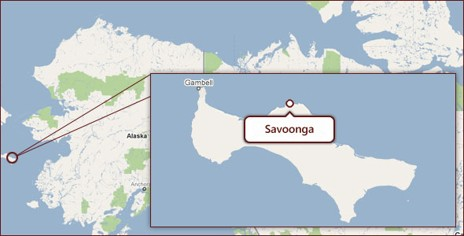
\includegraphics[width=0.8\linewidth,height=\textheight,keepaspectratio]{map.jpg}

}

\caption{\label{fig-map}Location of Savoonga, Alaska on St.~Lawrence
Island in the Bering Sea (Rosales et al. (2021)).}

\end{figure}%

Traditional Ecological Knowledge (TEK) refers to the environmental
knowledge and practices developed across generations through close
relationships with the land and observation of environmental changes
(Oregon State University Traditional Ecological Knowledge Lab (2026)).
In Arctic communities such as Savoonga, TEK plays an essential role in
understanding local weather patterns and guiding hunting and subsistence
activities. The Arctic region's extremely harsh environmental conditions
make it difficult to install and reliably maintain conventional
weather-monitoring equipment, such as wind sensors. As a result,
long-term instrumental records of local wind patterns that could have
been used to understand weather patterns or TEK recalibration are often
limited or unavailable. The cultural significance of TEK also makes it
essential to support its recalibration. TEK observations are qualitative
and long-term, often made by persons who hunt, fish, and gather for
subsistence. This makes TEK a part of a culture's spiritual and social
fabric, offering irreplaceable ecocultural knowledge that can be
thousands of years old and incorporates long-standing values (Oregon
State University Traditional Ecological Knowledge Lab (2026)).

Because of this significance of TEK in Arctic communities, a project by
Dr Rosales, Dr Ramler, and Dr Torrey at St.~Lawrence University proposes
to measure the TEK in Savoonga that the prevailing wind direction
changed from the historical northerly dominated winds 30 plus years ago
to southerly and easterly dominated winds around St.~Lawrence Island
(SLI), on which Savoonga is located. This will serve to recalibrate the
TEK of wind direction on SLI to restore the knowledge and practice of
observing wind direction that is being lost with a changing Arctic
(Rosales et al. (2021)).

It is for this project that tundra grasses were grown and studied at the
St.~Lawrence University Living Laboratory (SLU Living Lab) to serve as a
controlled and accessible proxy for field conditions in Savoonga.
Figure~\ref{fig-lab} shows images of the SLU Living Lab. The SLU Living
Lab is a 127-acre outdoor research and teaching site located near the
St.~Lawrence University campus in Canton, New York. The site includes
fields, forests, wetlands, and open grassland areas that support
environmental monitoring and ecological research (St. Lawrence
University (2026a)). Although the SLU Living Lab is not an Arctic
environment, it still experiences harsh winters and strong seasonal
variation, meaning the grass growing cycle is constrained in ways that
are somewhat comparable to tundra conditions, even if milder. Because it
is difficult to repeatedly measure wind conditions in the remote and
harsh environment of St.~Lawrence Island, the SLU Living Lab provides a
setting where wind data can be collected more systematically using wind
sensors while still mimicking similar and relevant environmental
constraints tundra grasses may face in the Savoonga region. This makes
it possible to test and refine image-based methods against collected
wind data for application to field-based TEK observations.

\begin{figure}[H]

\begin{minipage}[t]{0.50\linewidth}

\centering{

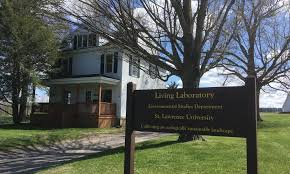
\includegraphics[width=0.85\linewidth,height=\textheight,keepaspectratio]{livinglab.jpg}

}

\subcaption{\label{fig-livinglab}}

\end{minipage}%
%
\begin{minipage}[t]{0.50\linewidth}

\centering{

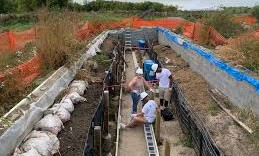
\includegraphics[width=0.85\linewidth,height=\textheight,keepaspectratio]{livinglab2.jpg}

}

\subcaption{\label{fig-livinglab2}}

\end{minipage}%

\caption{\label{fig-lab}Images of the SLU Living Lab (St. Lawrence
University (2026b)).}

\end{figure}%

In the Savoonga region, residents employ the TEK practice of observing
wind dynamics affecting tundra plants and in particular they examine
bluejoint reedgrass (Calamagrostis canadensis) and tall cottongrass
(Eriophorum angustifolium), in the sedge family, as indicators of
predominant wind direction and wind direction. Hunters and gatherers
from Savoonga observe the direction these plants lay down after the
growing season as proxies for predominant wind direction and wind
direction change (Rosales et al. (2021)). Preliminary work on this
project involved a manual process for estimating grass orientation from
field from the SLU Living Lab images. For instance, quadrat plots would
be outlined on the ground using meter-by-meter PVC frames oriented to
geographic north as shown in Figure~\ref{fig-compass}. Each quadrat was
photographed, and grass lay direction was then manually determined by
tracing the orientation of individual grass blades in the image.

\begin{figure}[H]

\centering{

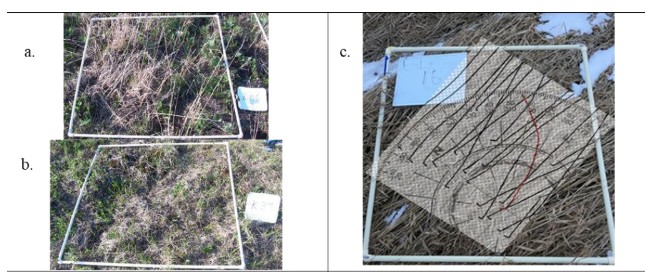
\includegraphics[width=0.8\linewidth,height=\textheight,keepaspectratio]{compass.jpg}

}

\caption{\label{fig-compass}Manual process for estimating grass
orientation in grass images (Rosales et al. (2021)).}

\end{figure}%

To support this manually strenuous process, we investigate how we can
use image gradient analysis techniques on the images of tundra grass
from the St.~Lawrence University Living Laboratory to automate the
process of measuring grass lay directions and determining their
association with collected wind data.

\clearpage

\section{Data}\label{data}

To evaluate this gradient analysis technique's performance, we used data
from the St.~Lawrence University Living Laboratory (SLU Living Lab).
From the SLU Living Lab, we collected 65 tundra grass images taken in
April 2023. The images taken were aerial images taken using a drone, see
some samples in Figure~\ref{fig-grasses}. There is a varied range of
images from a birds-eye view to close-up shots. Increasing variability
in the analysis, there are images with different kinds of noise such as
obstructing objects on land and buildings. Figure~\ref{fig-grasses}
displays the variability that may exist in each image. The red circles
on these images display the different directions that could be perceived
as dominant grass direction in the images.

\begin{figure}[H]

\begin{minipage}[t]{0.33\linewidth}

\centering{

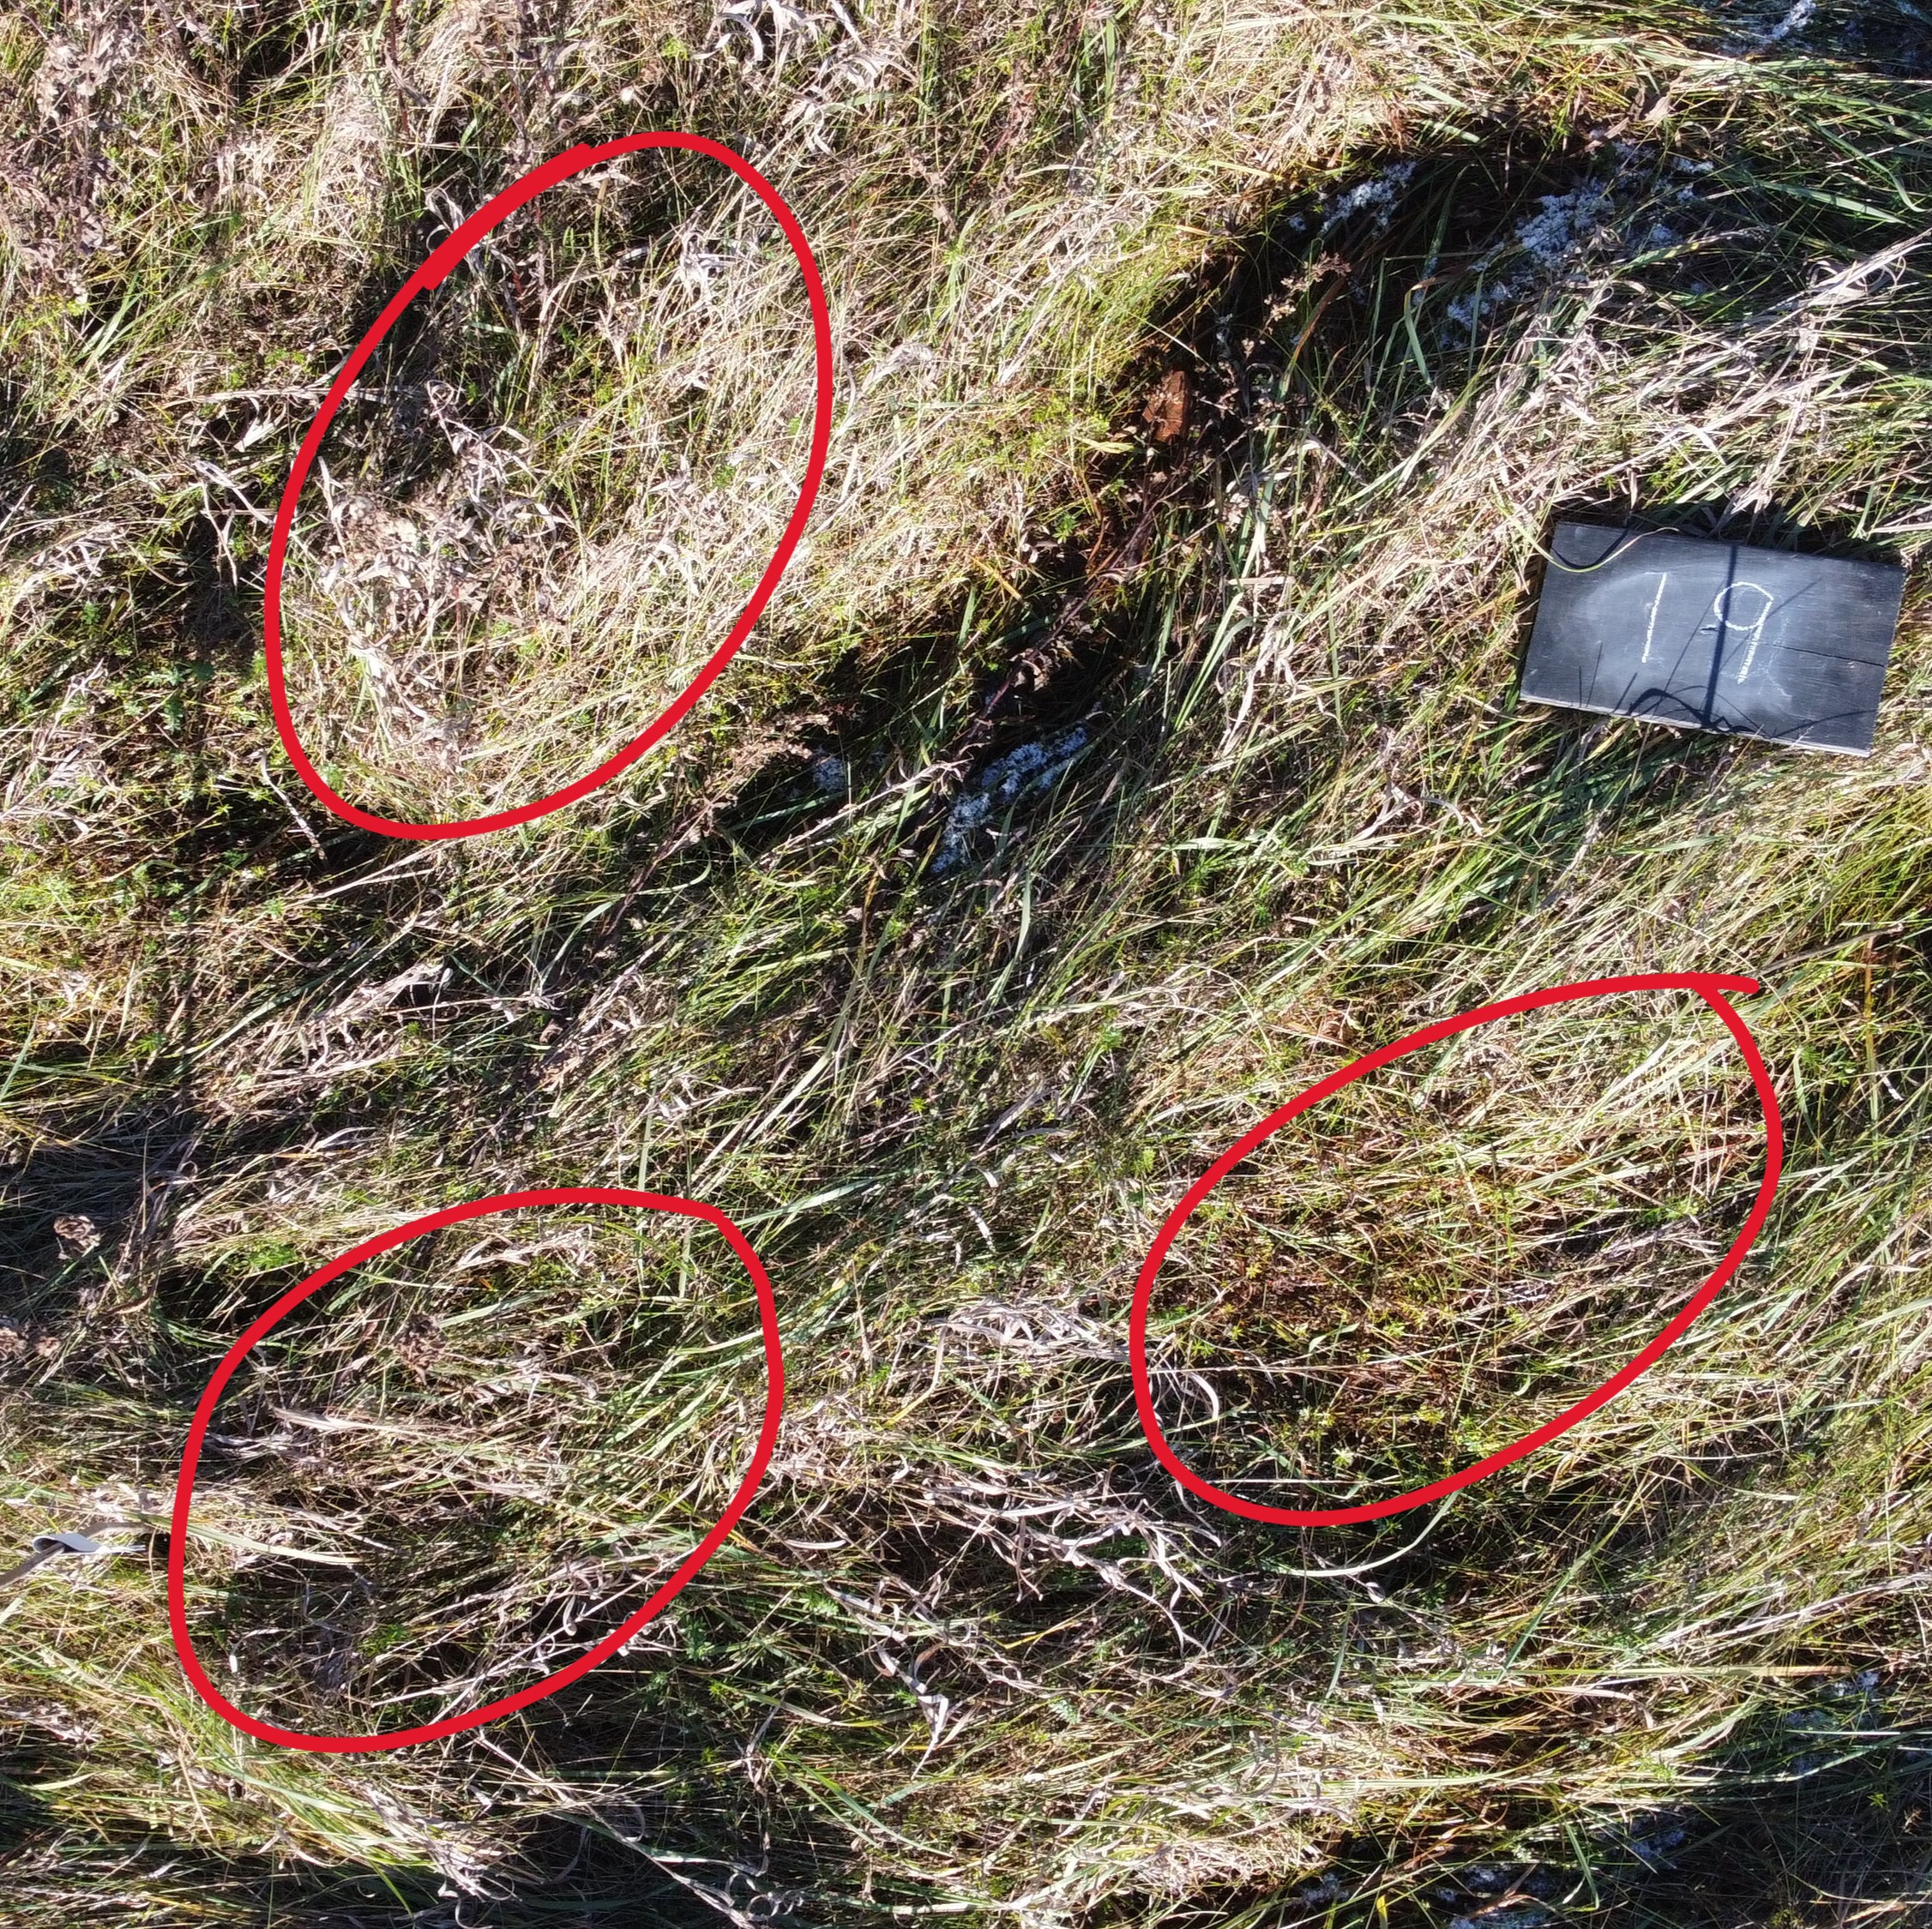
\includegraphics[width=0.9\linewidth,height=\textheight,keepaspectratio]{DJI_0256.JPG}

}

\subcaption{\label{fig-grass1}}

\end{minipage}%
%
\begin{minipage}[t]{0.33\linewidth}

\centering{

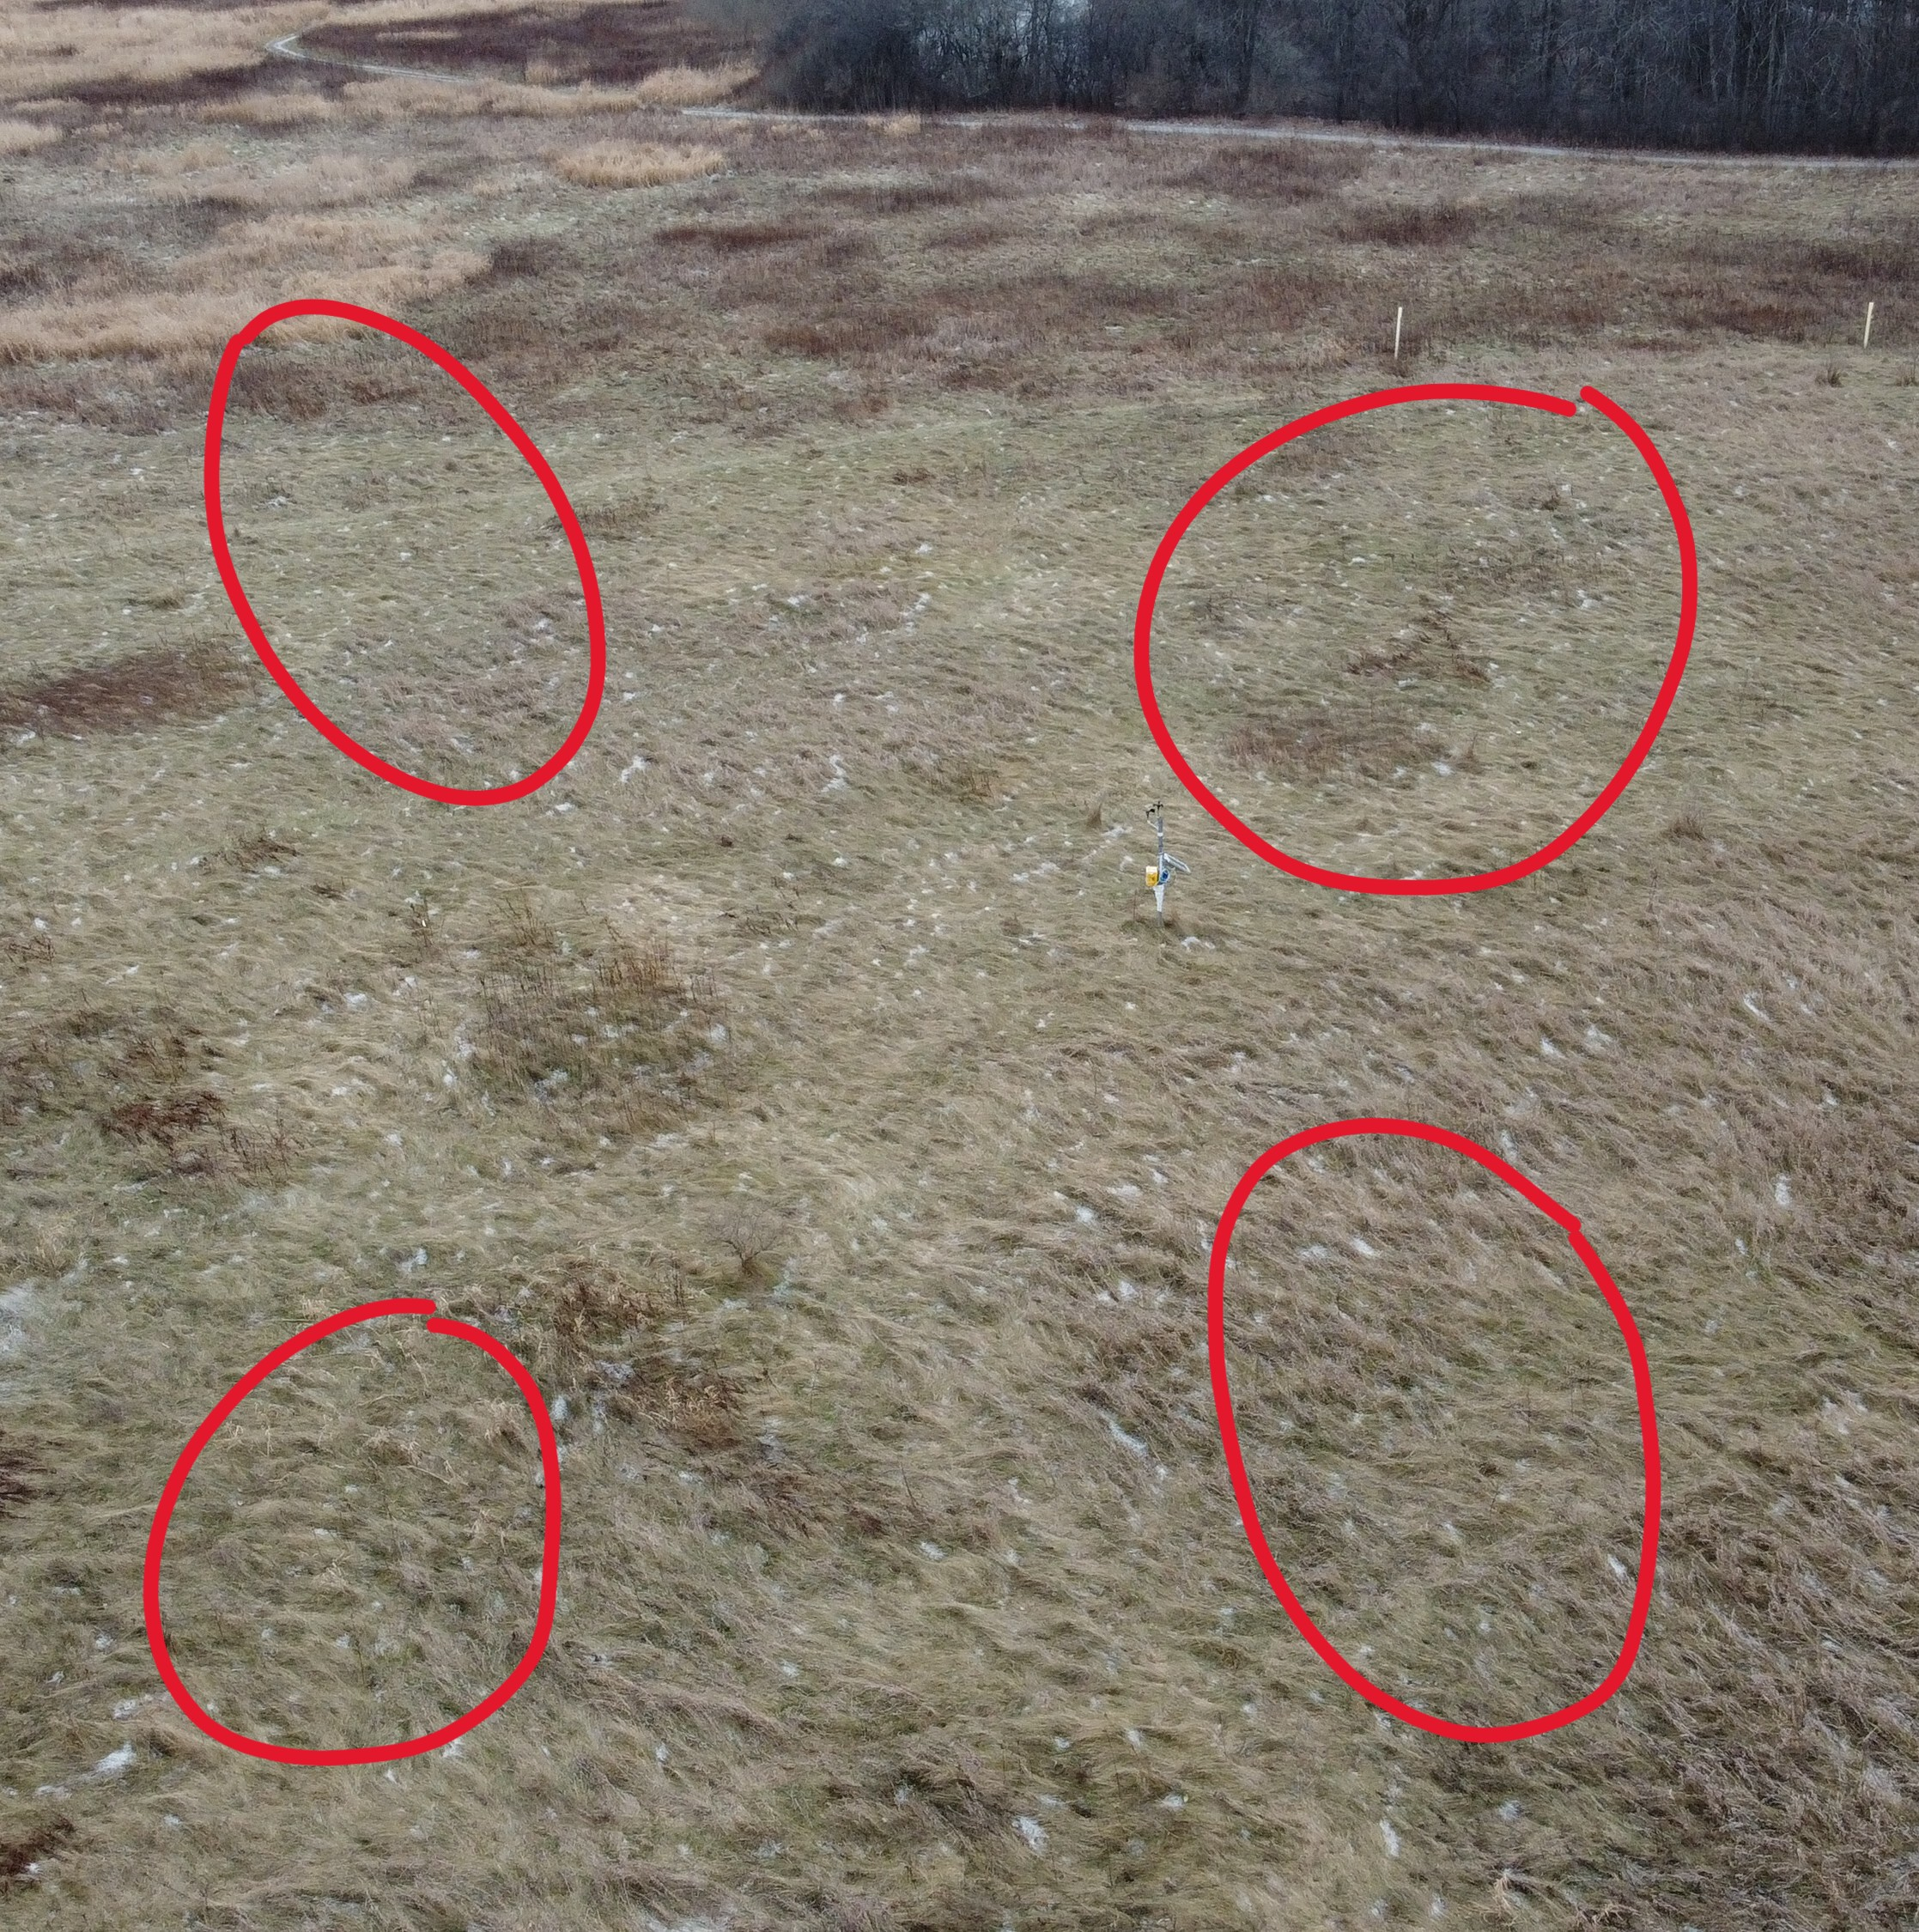
\includegraphics[width=0.9\linewidth,height=\textheight,keepaspectratio]{LL_grass.JPG}

}

\subcaption{\label{fig-grass2}}

\end{minipage}%
%
\begin{minipage}[t]{0.33\linewidth}

\centering{

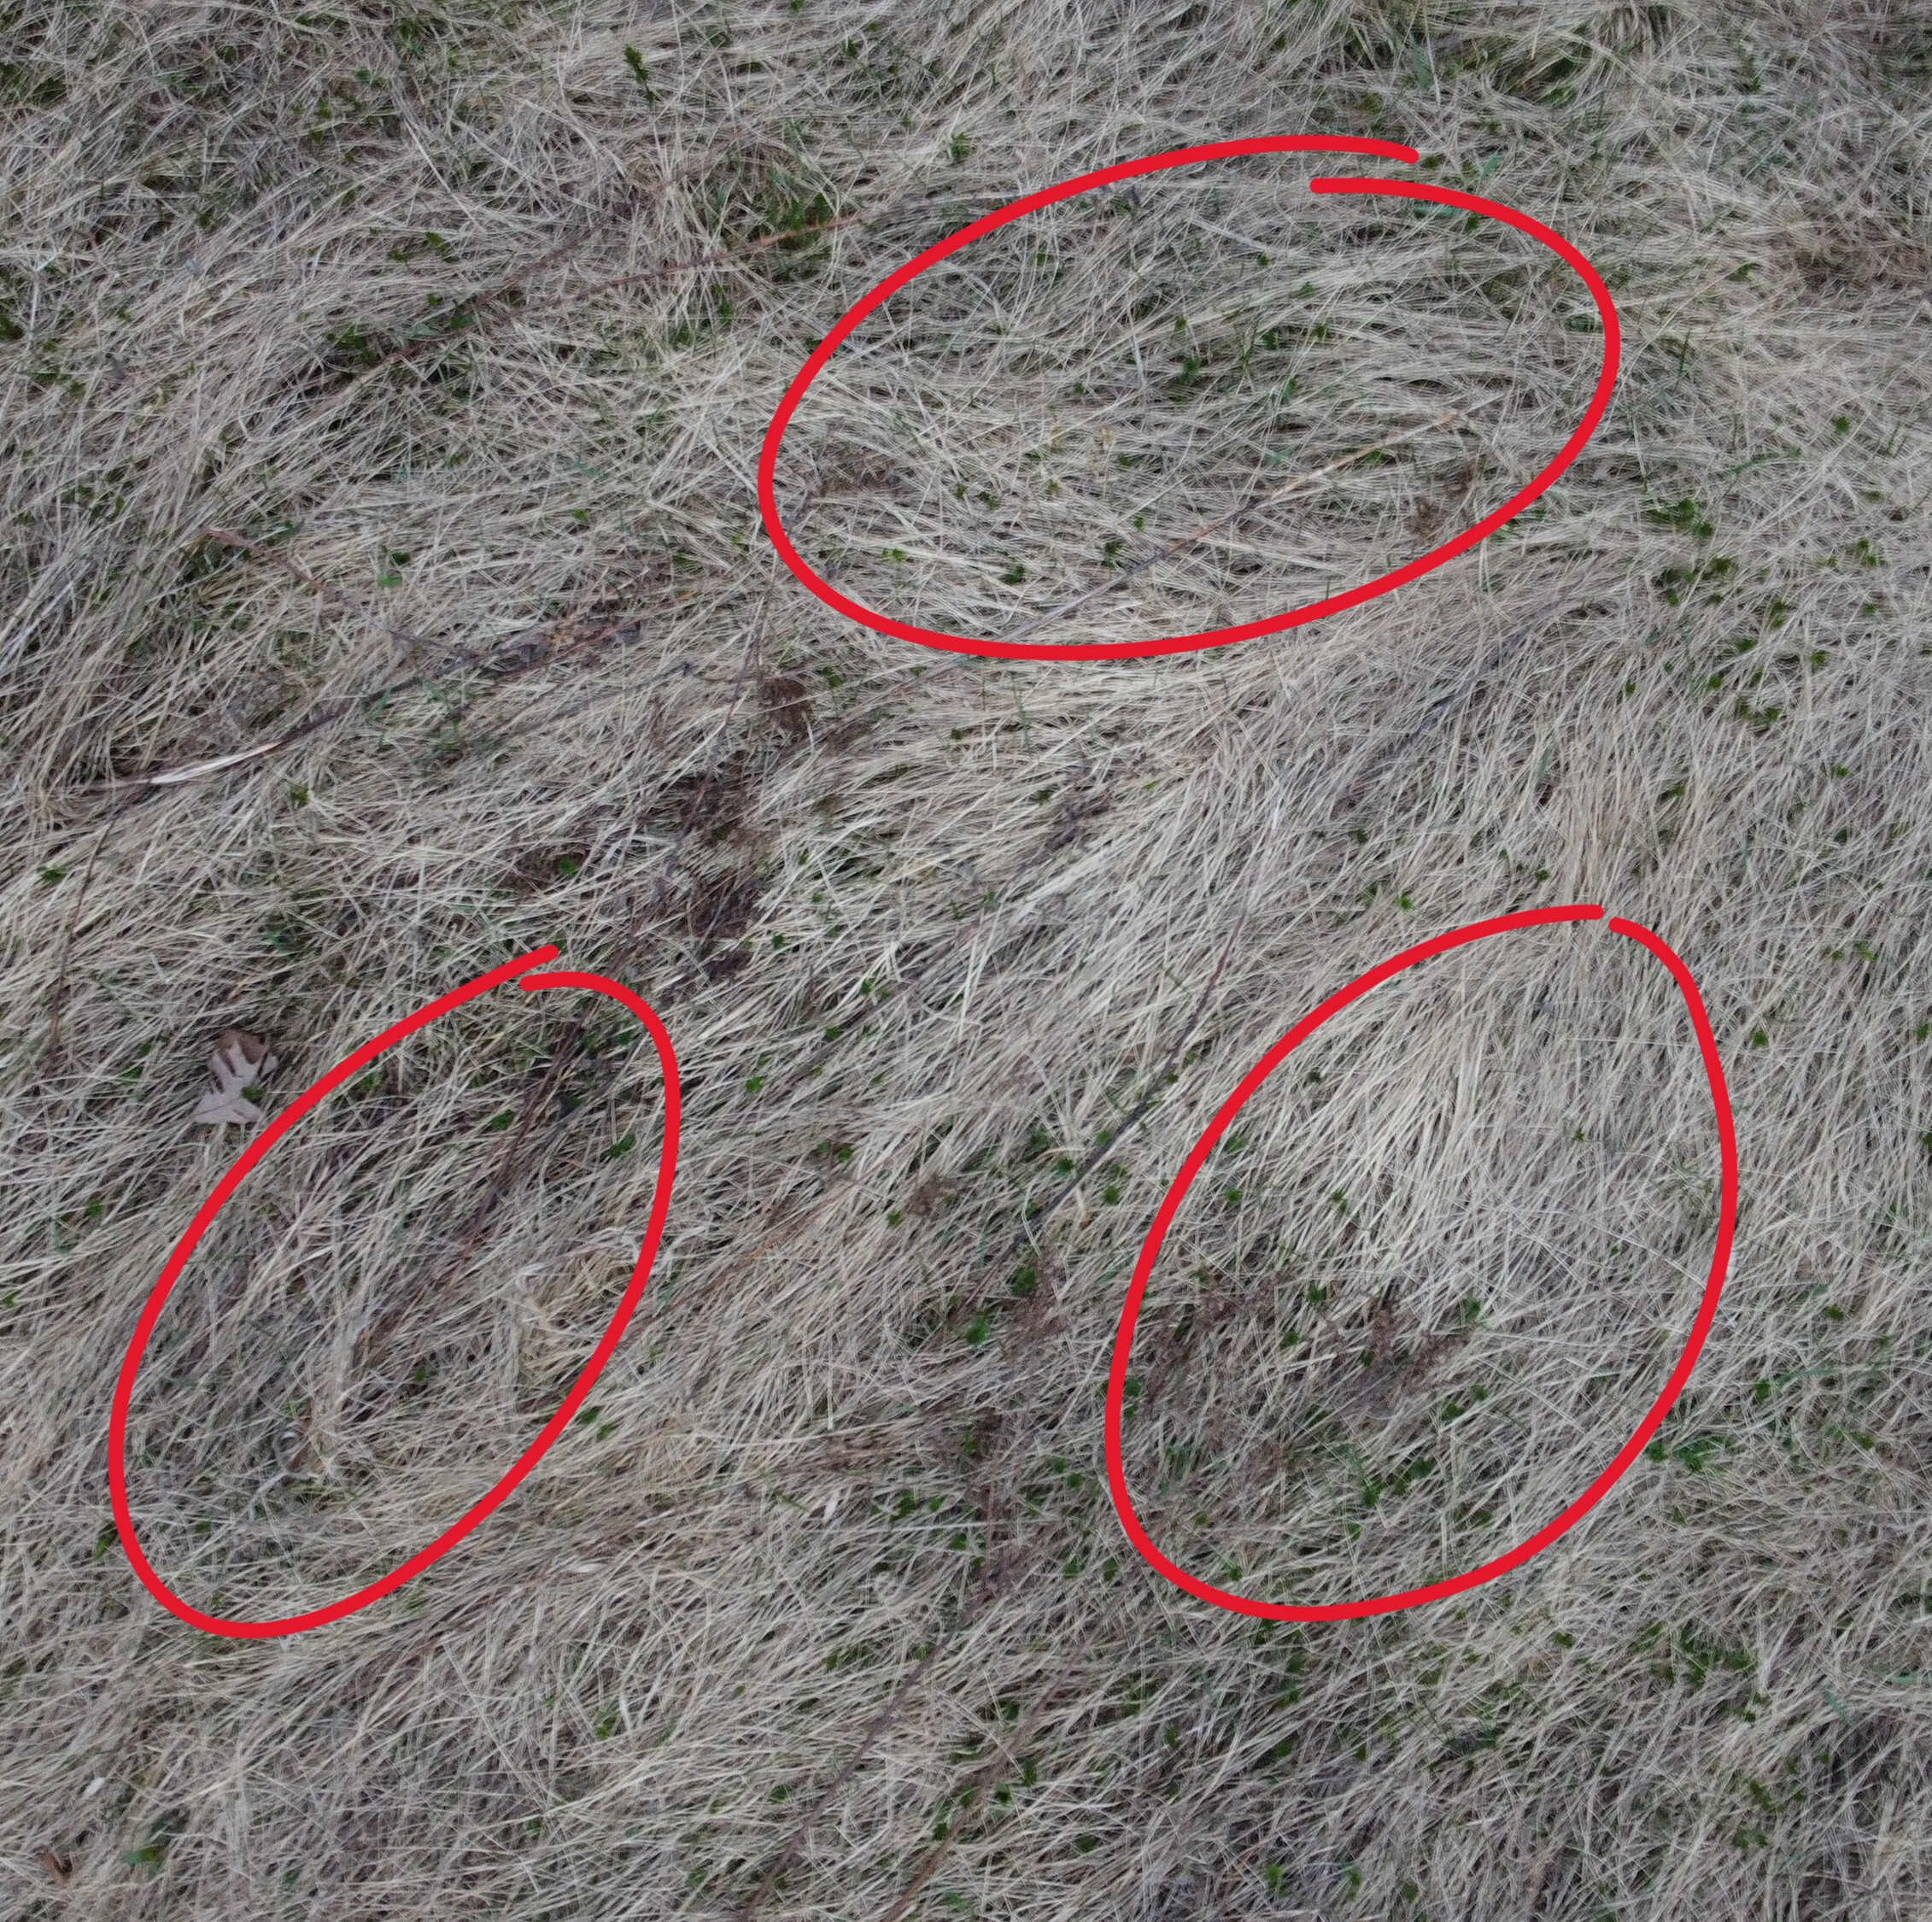
\includegraphics[width=0.9\linewidth,height=\textheight,keepaspectratio]{DJI_0358.JPG}

}

\subcaption{\label{fig-grass3}}

\end{minipage}%

\caption{\label{fig-grasses}Sample SLU Living Lab Drone Grass Images.
Source: Dr.~Jon Rosales.}

\end{figure}%

The SLU Living Lab also collects various weather data. The lab has an
installation of weather equipment that as seen in
Figure~\ref{fig-equipment}, retrieves data from a wind vane, anemometer,
and solar panel. This collects information about wind direction, speed,
and other atmospheric characteristics. This data is logged every 15
minutes. Table~\ref{tbl-winddata} is a table showing a snippet of the
wind data collected.

\begin{figure}[H]

\begin{minipage}[t]{0.51\linewidth}

\centering{

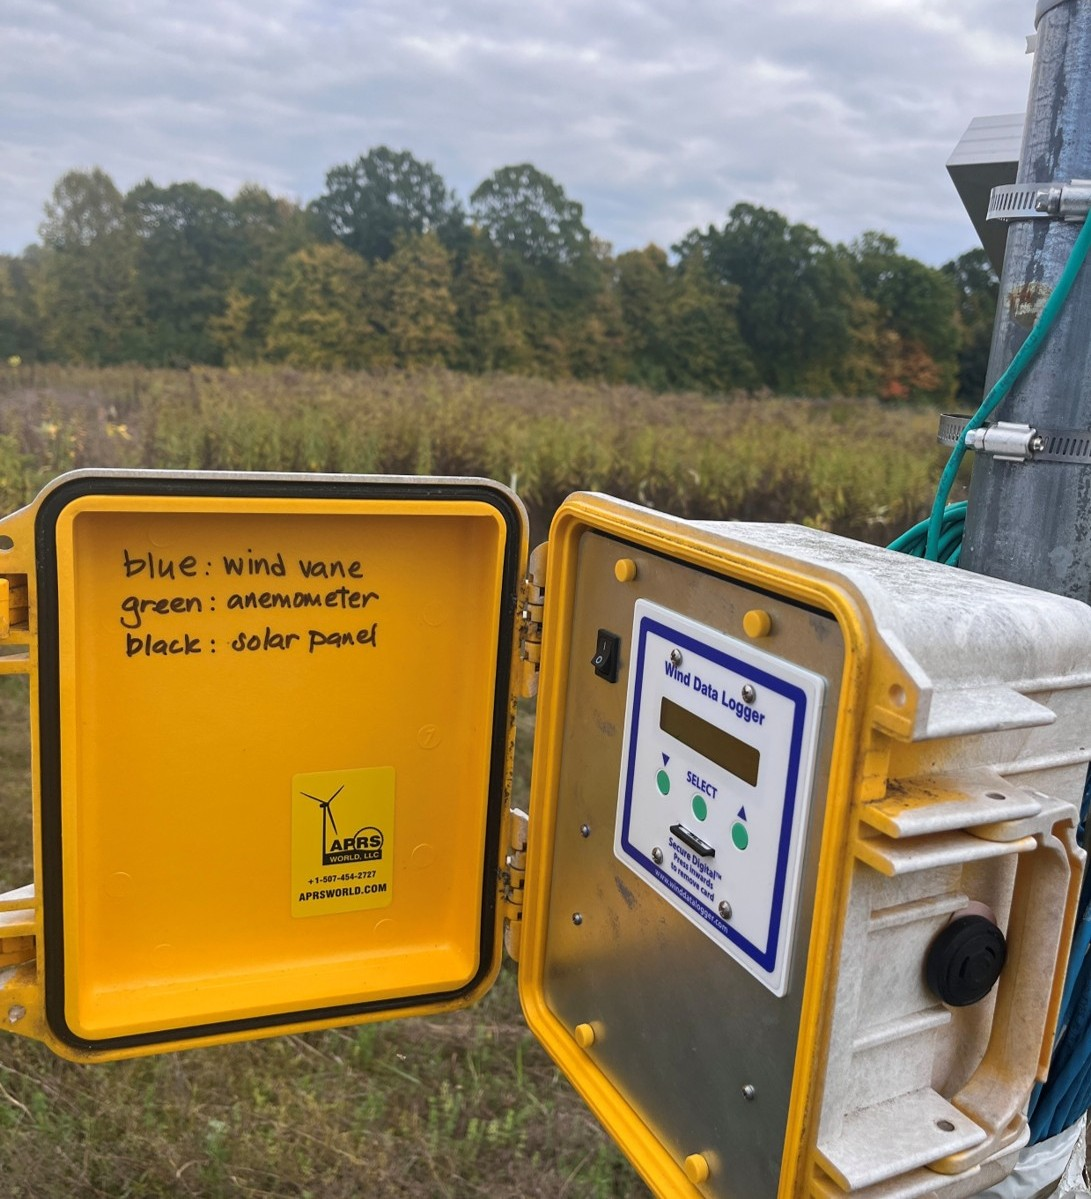
\includegraphics[width=0.6\linewidth,height=\textheight,keepaspectratio]{weatherequip.jpg}

}

\subcaption{\label{fig-equip1}}

\end{minipage}%
%
\begin{minipage}[t]{0.49\linewidth}

\centering{

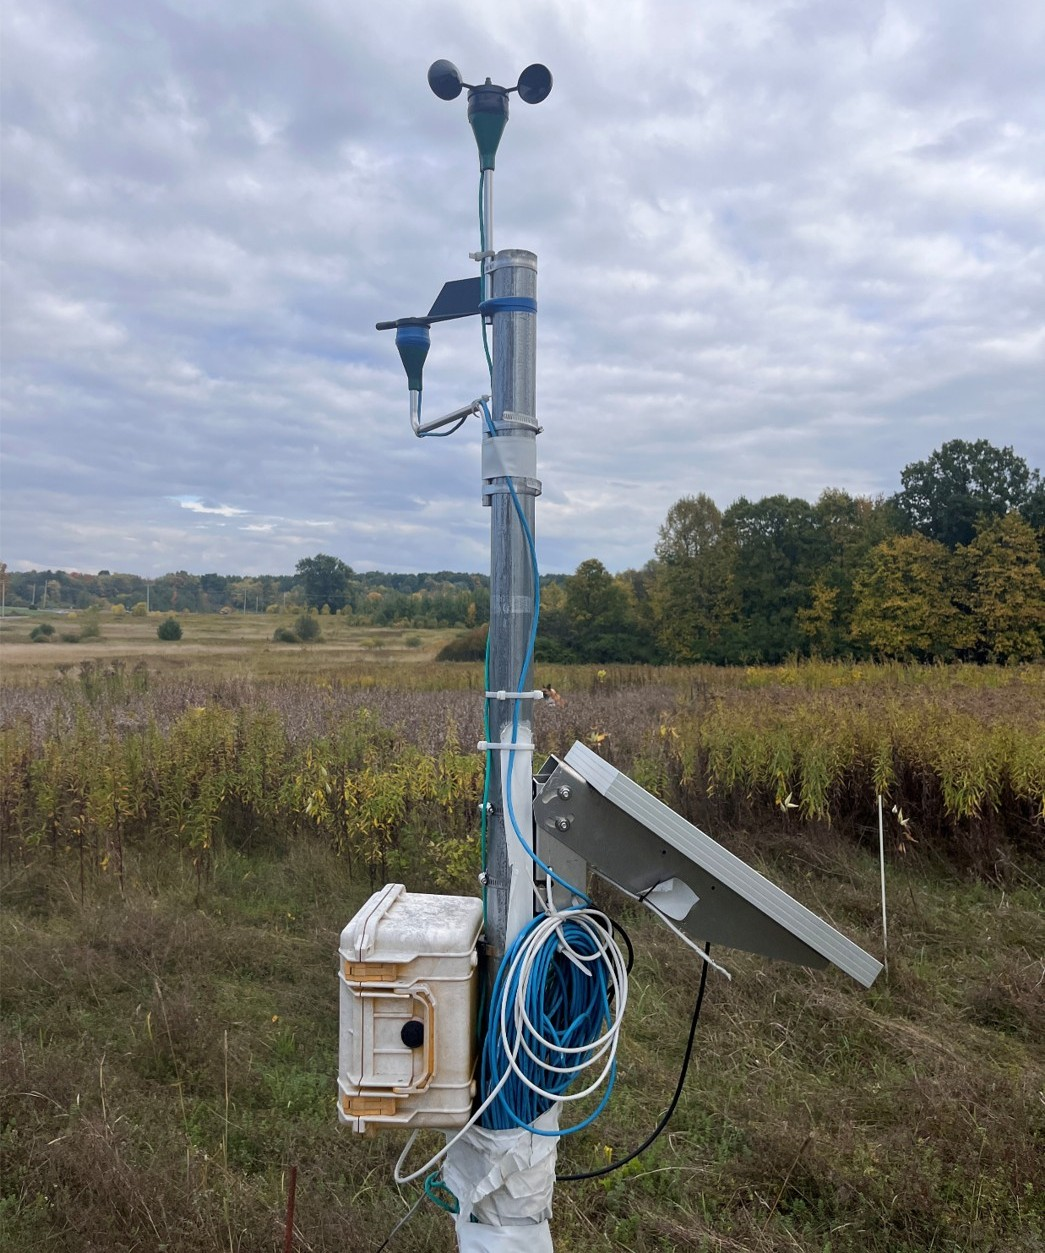
\includegraphics[width=0.57\linewidth,height=\textheight,keepaspectratio]{weatherequip2.jpg}

}

\subcaption{\label{fig-equip2}}

\end{minipage}%

\caption{\label{fig-equipment}Weather Equipment at the SLU Living Lab.}

\end{figure}%

\begin{table}

\caption{\label{tbl-winddata}}

\centering{

\centering
\begin{tabular}[t]{>{\raggedright\arraybackslash}p{4cm}>{\raggedleft\arraybackslash}p{4cm}>{\raggedleft\arraybackslash}p{4cm}}
\toprule
Date & Angle & Speed\\
\midrule
\cellcolor{gray!10}{2022-05-01 01:05:16} & \cellcolor{gray!10}{106} & \cellcolor{gray!10}{12.85}\\
2022-05-01 01:20:16 & 88 & 12.85\\
\cellcolor{gray!10}{2022-05-01 01:35:16} & \cellcolor{gray!10}{87} & \cellcolor{gray!10}{12.85}\\
2022-05-01 01:50:16 & 51 & 12.81\\
\cellcolor{gray!10}{2022-05-01 02:05:16} & \cellcolor{gray!10}{30} & \cellcolor{gray!10}{12.85}\\
\addlinespace
2022-05-01 02:20:16 & 76 & 12.85\\
\cellcolor{gray!10}{2022-05-01 02:35:16} & \cellcolor{gray!10}{337} & \cellcolor{gray!10}{12.81}\\
2022-05-01 02:50:16 & 319 & 12.81\\
\cellcolor{gray!10}{2022-05-01 03:05:16} & \cellcolor{gray!10}{288} & \cellcolor{gray!10}{12.81}\\
2022-05-01 03:20:16 & 305 & 12.81\\
\addlinespace
\cellcolor{gray!10}{2022-05-01 03:35:16} & \cellcolor{gray!10}{12} & \cellcolor{gray!10}{12.81}\\
\bottomrule
\end{tabular}

}

\end{table}%

\clearpage

\section{Methods}\label{methods}

\subsection{Gradient Analysis
Techniques}\label{gradient-analysis-techniques}

In a previous senior year research project, Ben Sunshine (Sunshine
(2024)) investigated the Histogram of Oriented Gradients (HOG) algorithm
to automate the measurement of grass lay angles. They applied the
algorithm to various images sampled from the internet and grass images
from the SLU Living Lab to test the algorithm's viability. Upon their
uncovering of its viability, this current project proceeds with adapting
the algorithm's gradient analysis techniques. The HOG algorithm, is a
method that is used to capture the orientation of textures in an image.
The first component of the HOG algorithm is to analyse gradients. An
image is split into small patches called cells, and we compute the
gradient magnitude and direction in each cell (Manavalan (2020)). These
local gradients, magnitudes, and angles are extracted and then
aggregated into vectors that describe the overall image to represent it
into patterns that identify images and their texture.
Figure~\ref{fig-hog} shows the raw grass image as the input, a grayscale
image that is broken down into cells, and a snippet of vectors
describing gradients in each cell of the image.

\begin{figure}[H]

\begin{minipage}[t]{0.50\linewidth}

\centering{

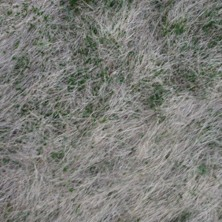
\includegraphics[width=0.65\linewidth,height=\textheight,keepaspectratio]{media/rawhog.jpg}

}

\subcaption{\label{fig-raw}Input Grass Image}

\end{minipage}%
%
\begin{minipage}[t]{0.50\linewidth}

\centering{

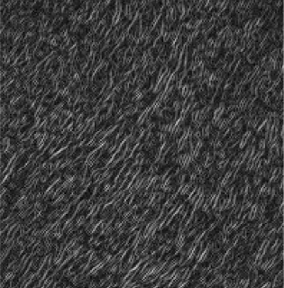
\includegraphics[width=0.65\linewidth,height=\textheight,keepaspectratio]{media/posthog.png}

}

\subcaption{\label{fig-posthog}Grayscaled and Decomposed Grass Image}

\end{minipage}%
\newline
\begin{minipage}[t]{\linewidth}
~\end{minipage}%
\newline
\begin{minipage}[t]{\linewidth}

\centering{

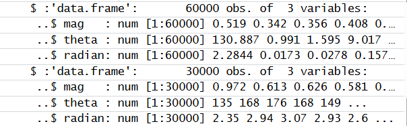
\includegraphics[width=0.7\linewidth,height=\textheight,keepaspectratio]{media/vechog.png}

}

\subcaption{\label{fig-df}Snippet of Vectors Describing Grass Image}

\end{minipage}%

\caption{\label{fig-hog}Steps of HOG Gradient Analysis.}

\end{figure}%

While the full HOG algorithm divides images into structured cells and
further aggregates gradients into histograms, this study focuses on the
core component of the method that extracts pixel-level gradient angles
and magnitudes to capture dominant directions in grass images.

The preliminary processing of the gradient analysis included loading
several R packages to support image manipulation, data handling, and
statistical analysis, including \texttt{tidyverse}, \texttt{imager},
\texttt{magick}, \texttt{tectonicr}, and \texttt{exif}.

\begin{Shaded}
\begin{Highlighting}[]
\FunctionTok{library}\NormalTok{(tidyverse)}
\FunctionTok{library}\NormalTok{(magick)}
\FunctionTok{library}\NormalTok{(imager)}
\FunctionTok{library}\NormalTok{(readr)}
\FunctionTok{library}\NormalTok{(exif)}
\FunctionTok{library}\NormalTok{(tectonicr)}
\end{Highlighting}
\end{Shaded}

For each image, the processing included loading, converting the image to
grayscale, and resizing it. Images were rescaled to a fixed height while
preserving their aspect ratio to ensure consistent resolution across all
images without introducing geometric distortion. The images were
converted to grayscale to allow for focusing on representing pixel
intensity in terms of texture and structural variation, rather than
color information.

\begin{Shaded}
\begin{Highlighting}[]
\NormalTok{  img }\OtherTok{\textless{}{-}} \FunctionTok{load.image}\NormalTok{(image) }\CommentTok{\# load the image being viewed now}
\NormalTok{  img\_gray }\OtherTok{\textless{}{-}} \FunctionTok{grayscale}\NormalTok{(img) }\CommentTok{\# convert to gray scale}
\NormalTok{  dims }\OtherTok{\textless{}{-}} \FunctionTok{dim}\NormalTok{(img\_gray) }\CommentTok{\# retrieve dimensions of the grayed image}
\NormalTok{  h0 }\OtherTok{\textless{}{-}}\NormalTok{ dims[}\DecValTok{1}\NormalTok{] }\CommentTok{\# the height}
\NormalTok{  w0 }\OtherTok{\textless{}{-}}\NormalTok{ dims[}\DecValTok{2}\NormalTok{] }\CommentTok{\# the width}
  
  \CommentTok{\# resize to target height to keep consistent size of images}
\NormalTok{  target\_height }\OtherTok{\textless{}{-}} \DecValTok{200} 
\NormalTok{  target\_width }\OtherTok{\textless{}{-}} \FunctionTok{max}\NormalTok{(}\DecValTok{1}\NormalTok{, }\FunctionTok{round}\NormalTok{(w0 }\SpecialCharTok{*}\NormalTok{ (target\_height }\SpecialCharTok{/}\NormalTok{ h0))) }
  \CommentTok{\# relative to target\_height}
  \CommentTok{\# recalculate width to maintain same aspect ratio}
\NormalTok{  img\_resized }\OtherTok{\textless{}{-}} \FunctionTok{resize}\NormalTok{(img\_gray, }\AttributeTok{size\_x =}\NormalTok{ target\_width, }
  \AttributeTok{size\_y =}\NormalTok{ target\_height)}
\end{Highlighting}
\end{Shaded}

The processed image is stored as \texttt{M}. The image's structure is
defined by rows and columns of pixel values. Because the \texttt{imager}
package loads images as 4-dimensional arrays by default (width, height,
depth, and color channels), the image is first reduced to a 2D matrix by
extracting only two channels, since the grayscale image contains no
color or depth information that would require additional dimensions. The
dimensions of \texttt{M} are used to define image size, where \texttt{h}
represents the number of pixel rows which is the height of the image and
\texttt{w} which represents the number of pixel columns that is the
width of the image.

\begin{Shaded}
\begin{Highlighting}[]
\NormalTok{  M }\OtherTok{\textless{}{-}}\NormalTok{ img\_resized}
  
  \CommentTok{\# ensures the resized grayscale image is a 2D matrix}
  \ControlFlowTok{if}\NormalTok{ (}\FunctionTok{length}\NormalTok{(}\FunctionTok{dim}\NormalTok{(M)) }\SpecialCharTok{==} \DecValTok{4}\NormalTok{) }
\NormalTok{    M }\OtherTok{\textless{}{-}}\NormalTok{ M[,,}\DecValTok{1}\NormalTok{,}\DecValTok{1}\NormalTok{]}
  
\NormalTok{  M }\OtherTok{\textless{}{-}} \FunctionTok{as.matrix}\NormalTok{(M)}
  
  \CommentTok{\# how many rows and cols of pixels in the images}
\NormalTok{  h }\OtherTok{\textless{}{-}} \FunctionTok{nrow}\NormalTok{(M) }
\NormalTok{  w }\OtherTok{\textless{}{-}} \FunctionTok{ncol}\NormalTok{(M)}
\end{Highlighting}
\end{Shaded}

The gradient magnitudes and angles were then computed for every pixel in
the resized image. At each pixel at row \texttt{i} and column
\texttt{j}, the gradient is measured in two directions. The horizontal
gradient, \texttt{Gx}, is computed by taking the difference between the
pixel values immediately to the right \texttt{M{[}i,\ j+1{]}} and left
\texttt{M{[}i,\ j-1{]}} of the pixel of interest. The vertical gradient,
\texttt{Gy}, is computed by taking the difference between the pixel
value below \texttt{M{[}i+1,\ j{]}} and the pixel value above
\texttt{M{[}i-1,\ j{]}} it. At image boundaries where a neighboring
pixel does not exist on one side, a one-sided difference is used
instead. The overall gradient magnitude at each pixel is then derived by
combining \texttt{Gx} and \texttt{Gy} using the Pythagorean formula,
\(\text{mag} = \sqrt{G_x^2 + G_y^2}\), which captures the strength of
the intensity change at that location regardless of direction. The
gradient angle is computed using the arctangent of the ratio of
\texttt{Gy} to \texttt{Gx}, converted from radians to degrees.

\begin{Shaded}
\begin{Highlighting}[]
\ControlFlowTok{for}\NormalTok{ (i }\ControlFlowTok{in} \DecValTok{1}\SpecialCharTok{:}\NormalTok{h) \{}
  \ControlFlowTok{for}\NormalTok{ (j }\ControlFlowTok{in} \DecValTok{1}\SpecialCharTok{:}\NormalTok{w) \{}

\NormalTok{    Gx }\OtherTok{\textless{}{-}} \ControlFlowTok{if}\NormalTok{ (j }\SpecialCharTok{==} \DecValTok{1}\NormalTok{) M[i, j}\SpecialCharTok{+}\DecValTok{1}\NormalTok{] }
          \ControlFlowTok{else} \ControlFlowTok{if}\NormalTok{ (j }\SpecialCharTok{==}\NormalTok{ w) }\SpecialCharTok{{-}}\NormalTok{M[i, j}\DecValTok{{-}1}\NormalTok{] }
          \ControlFlowTok{else}\NormalTok{ M[i, j}\SpecialCharTok{+}\DecValTok{1}\NormalTok{] }\SpecialCharTok{{-}}\NormalTok{ M[i, j}\DecValTok{{-}1}\NormalTok{]}

\NormalTok{    Gy }\OtherTok{\textless{}{-}} \ControlFlowTok{if}\NormalTok{ (i }\SpecialCharTok{==} \DecValTok{1}\NormalTok{) }\SpecialCharTok{{-}}\NormalTok{M[i}\SpecialCharTok{+}\DecValTok{1}\NormalTok{, j] }
          \ControlFlowTok{else} \ControlFlowTok{if}\NormalTok{ (i }\SpecialCharTok{==}\NormalTok{ h) M[i}\DecValTok{{-}1}\NormalTok{, j] }
          \ControlFlowTok{else}\NormalTok{ M[i}\SpecialCharTok{+}\DecValTok{1}\NormalTok{, j] }\SpecialCharTok{{-}}\NormalTok{ M[i}\DecValTok{{-}1}\NormalTok{, j]}

\NormalTok{    mag }\OtherTok{\textless{}{-}} \FunctionTok{sqrt}\NormalTok{(Gx}\SpecialCharTok{\^{}}\DecValTok{2} \SpecialCharTok{+}\NormalTok{ Gy}\SpecialCharTok{\^{}}\DecValTok{2}\NormalTok{)}
\NormalTok{  \}}
\NormalTok{\}}
\end{Highlighting}
\end{Shaded}

Grass blades are symmetric in appearance. This means that to the
algorithm, a blade pointing at 10° looks the same as one pointing at
190°. Because of this, within each pixel, angles are then mapped onto a
0°--180° range. Any negative angle resulting from the arctangent
calculation is shifted by adding 180° to bring it into this range.

\begin{Shaded}
\begin{Highlighting}[]
\NormalTok{angle }\OtherTok{\textless{}{-}} \ControlFlowTok{if}\NormalTok{ (Gx }\SpecialCharTok{==} \DecValTok{0}\NormalTok{) }\DecValTok{0} \ControlFlowTok{else} \FunctionTok{atan}\NormalTok{(Gy }\SpecialCharTok{/}\NormalTok{ Gx) }\SpecialCharTok{*} \DecValTok{180} \SpecialCharTok{/}\NormalTok{ pi}
\ControlFlowTok{if}\NormalTok{ (angle }\SpecialCharTok{\textless{}} \DecValTok{0}\NormalTok{) angle }\OtherTok{\textless{}{-}}\NormalTok{ angle }\SpecialCharTok{+} \DecValTok{180}
\end{Highlighting}
\end{Shaded}

These values are then stored as vectors and structured as datasets
describing each image. During computation, magnitudes and angles are
stored row by row into lists, \texttt{mag\_list} and
\texttt{theta\_list}, rather than directly into vectors. This is because
appending to a list in R is more efficient than growing a vector element
by element inside a nested loop, which would require R to copy and
reallocate memory at each iteration. Once all pixel rows have been
processed, the lists are converted to flat vectors using
\texttt{unlist()} and combined into a data frame with one row per pixel
containing the angle in degrees, the gradient magnitude, and the angle
converted to radians. Because grass blades have defined, fine, and
linear textures, these gradient extraction techniques effectively
identify dominant directions and magnitudes. This supports our ability
to capture a general trend or flow in the grass making gradient analysis
useful for identifying a dominant grass lay direction.

\begin{Shaded}
\begin{Highlighting}[]
\CommentTok{\# initialize lists to store the mags and theta}
\NormalTok{mag\_list }\OtherTok{\textless{}{-}} \FunctionTok{vector}\NormalTok{(}\StringTok{"list"}\NormalTok{, h)}
\NormalTok{theta\_list }\OtherTok{\textless{}{-}} \FunctionTok{vector}\NormalTok{(}\StringTok{"list"}\NormalTok{, h)}

\NormalTok{mag\_list[[i]] }\OtherTok{\textless{}{-}}\NormalTok{ mag\_row}
\NormalTok{theta\_list[[i]] }\OtherTok{\textless{}{-}}\NormalTok{ theta\_row}

\CommentTok{\# Convert to vectors + save to df}
\NormalTok{mag\_vec }\OtherTok{\textless{}{-}} \FunctionTok{unlist}\NormalTok{(mag\_list)}
\NormalTok{theta\_vec }\OtherTok{\textless{}{-}} \FunctionTok{unlist}\NormalTok{(theta\_list)}
\NormalTok{radian\_vec }\OtherTok{\textless{}{-}}\NormalTok{ theta\_vec }\SpecialCharTok{*}\NormalTok{ pi }\SpecialCharTok{/} \DecValTok{180}

\NormalTok{dataset\_df }\OtherTok{\textless{}{-}} \FunctionTok{data.frame}\NormalTok{(}
\AttributeTok{theta =}\NormalTok{ theta\_vec,}
\AttributeTok{mag =}\NormalTok{ mag\_vec,}
\AttributeTok{radian =}\NormalTok{ radian\_vec}
\NormalTok{)}
\end{Highlighting}
\end{Shaded}

To observe how this gradient analysis visualizes the dominant direction
of grass in an image, Figure~\ref{fig-gradientplots} shows a
side-by-side comparison of a raw grass image from the St.~Lawrence
University Living Laboratory and its corresponding polar plot. The polar
plot is generated by reading the per-pixel angle and magnitudes dataset
saved for that image and plotting the theta column as a circular
histogram using \texttt{ggplot2}'s coord\_polar(). Each bar represents
the count of pixels whose gradient angles fall within that direction,
with compass directions labeled around the outside. The direction of the
tallest bar represents the most frequently occurring gradient angle,
giving a visual impression of the dominant grass lay direction detected
by the algorithm.

\begin{Shaded}
\begin{Highlighting}[]
\NormalTok{df }\OtherTok{\textless{}{-}} \FunctionTok{read\_csv}\NormalTok{(}\StringTok{"../output/angles\_mags/DJI\_0362.csv"}\NormalTok{)}

\FunctionTok{ggplot}\NormalTok{(df, }\FunctionTok{aes}\NormalTok{(}\AttributeTok{x =}\NormalTok{ theta)) }\SpecialCharTok{+}
  \FunctionTok{geom\_histogram}\NormalTok{(}
    \AttributeTok{colour =} \StringTok{"black"}\NormalTok{, }
    \AttributeTok{fill =} \StringTok{"darkgreen"}\NormalTok{, }
    \AttributeTok{breaks =} \FunctionTok{seq}\NormalTok{(}\DecValTok{0}\NormalTok{, }\DecValTok{360}\NormalTok{, }\AttributeTok{length.out =} \FloatTok{17.5}\NormalTok{)}
\NormalTok{  ) }\SpecialCharTok{+}
  \FunctionTok{coord\_polar}\NormalTok{(}\AttributeTok{theta =} \StringTok{"x"}\NormalTok{, }\AttributeTok{start =} \DecValTok{0}\NormalTok{, }\AttributeTok{direction =} \DecValTok{1}\NormalTok{) }\SpecialCharTok{+}
  \FunctionTok{scale\_x\_continuous}\NormalTok{(}
    \AttributeTok{limits =} \FunctionTok{c}\NormalTok{(}\DecValTok{0}\NormalTok{, }\DecValTok{360}\NormalTok{),}
    \AttributeTok{breaks =} \FunctionTok{c}\NormalTok{(}\DecValTok{0}\NormalTok{, }\DecValTok{45}\NormalTok{, }\DecValTok{90}\NormalTok{, }\DecValTok{135}\NormalTok{, }\DecValTok{180}\NormalTok{, }\DecValTok{225}\NormalTok{, }\DecValTok{270}\NormalTok{, }\DecValTok{315}\NormalTok{),}
    \AttributeTok{labels =} \FunctionTok{c}\NormalTok{(}\StringTok{"N"}\NormalTok{, }\StringTok{"NE"}\NormalTok{, }\StringTok{"E"}\NormalTok{, }\StringTok{"SE"}\NormalTok{, }\StringTok{"S"}\NormalTok{, }\StringTok{"SW"}\NormalTok{, }\StringTok{"W"}\NormalTok{, }\StringTok{"NW"}\NormalTok{)}
\NormalTok{  )}
\end{Highlighting}
\end{Shaded}

\begin{figure}[H]

\begin{minipage}[t]{0.50\linewidth}

\centering{

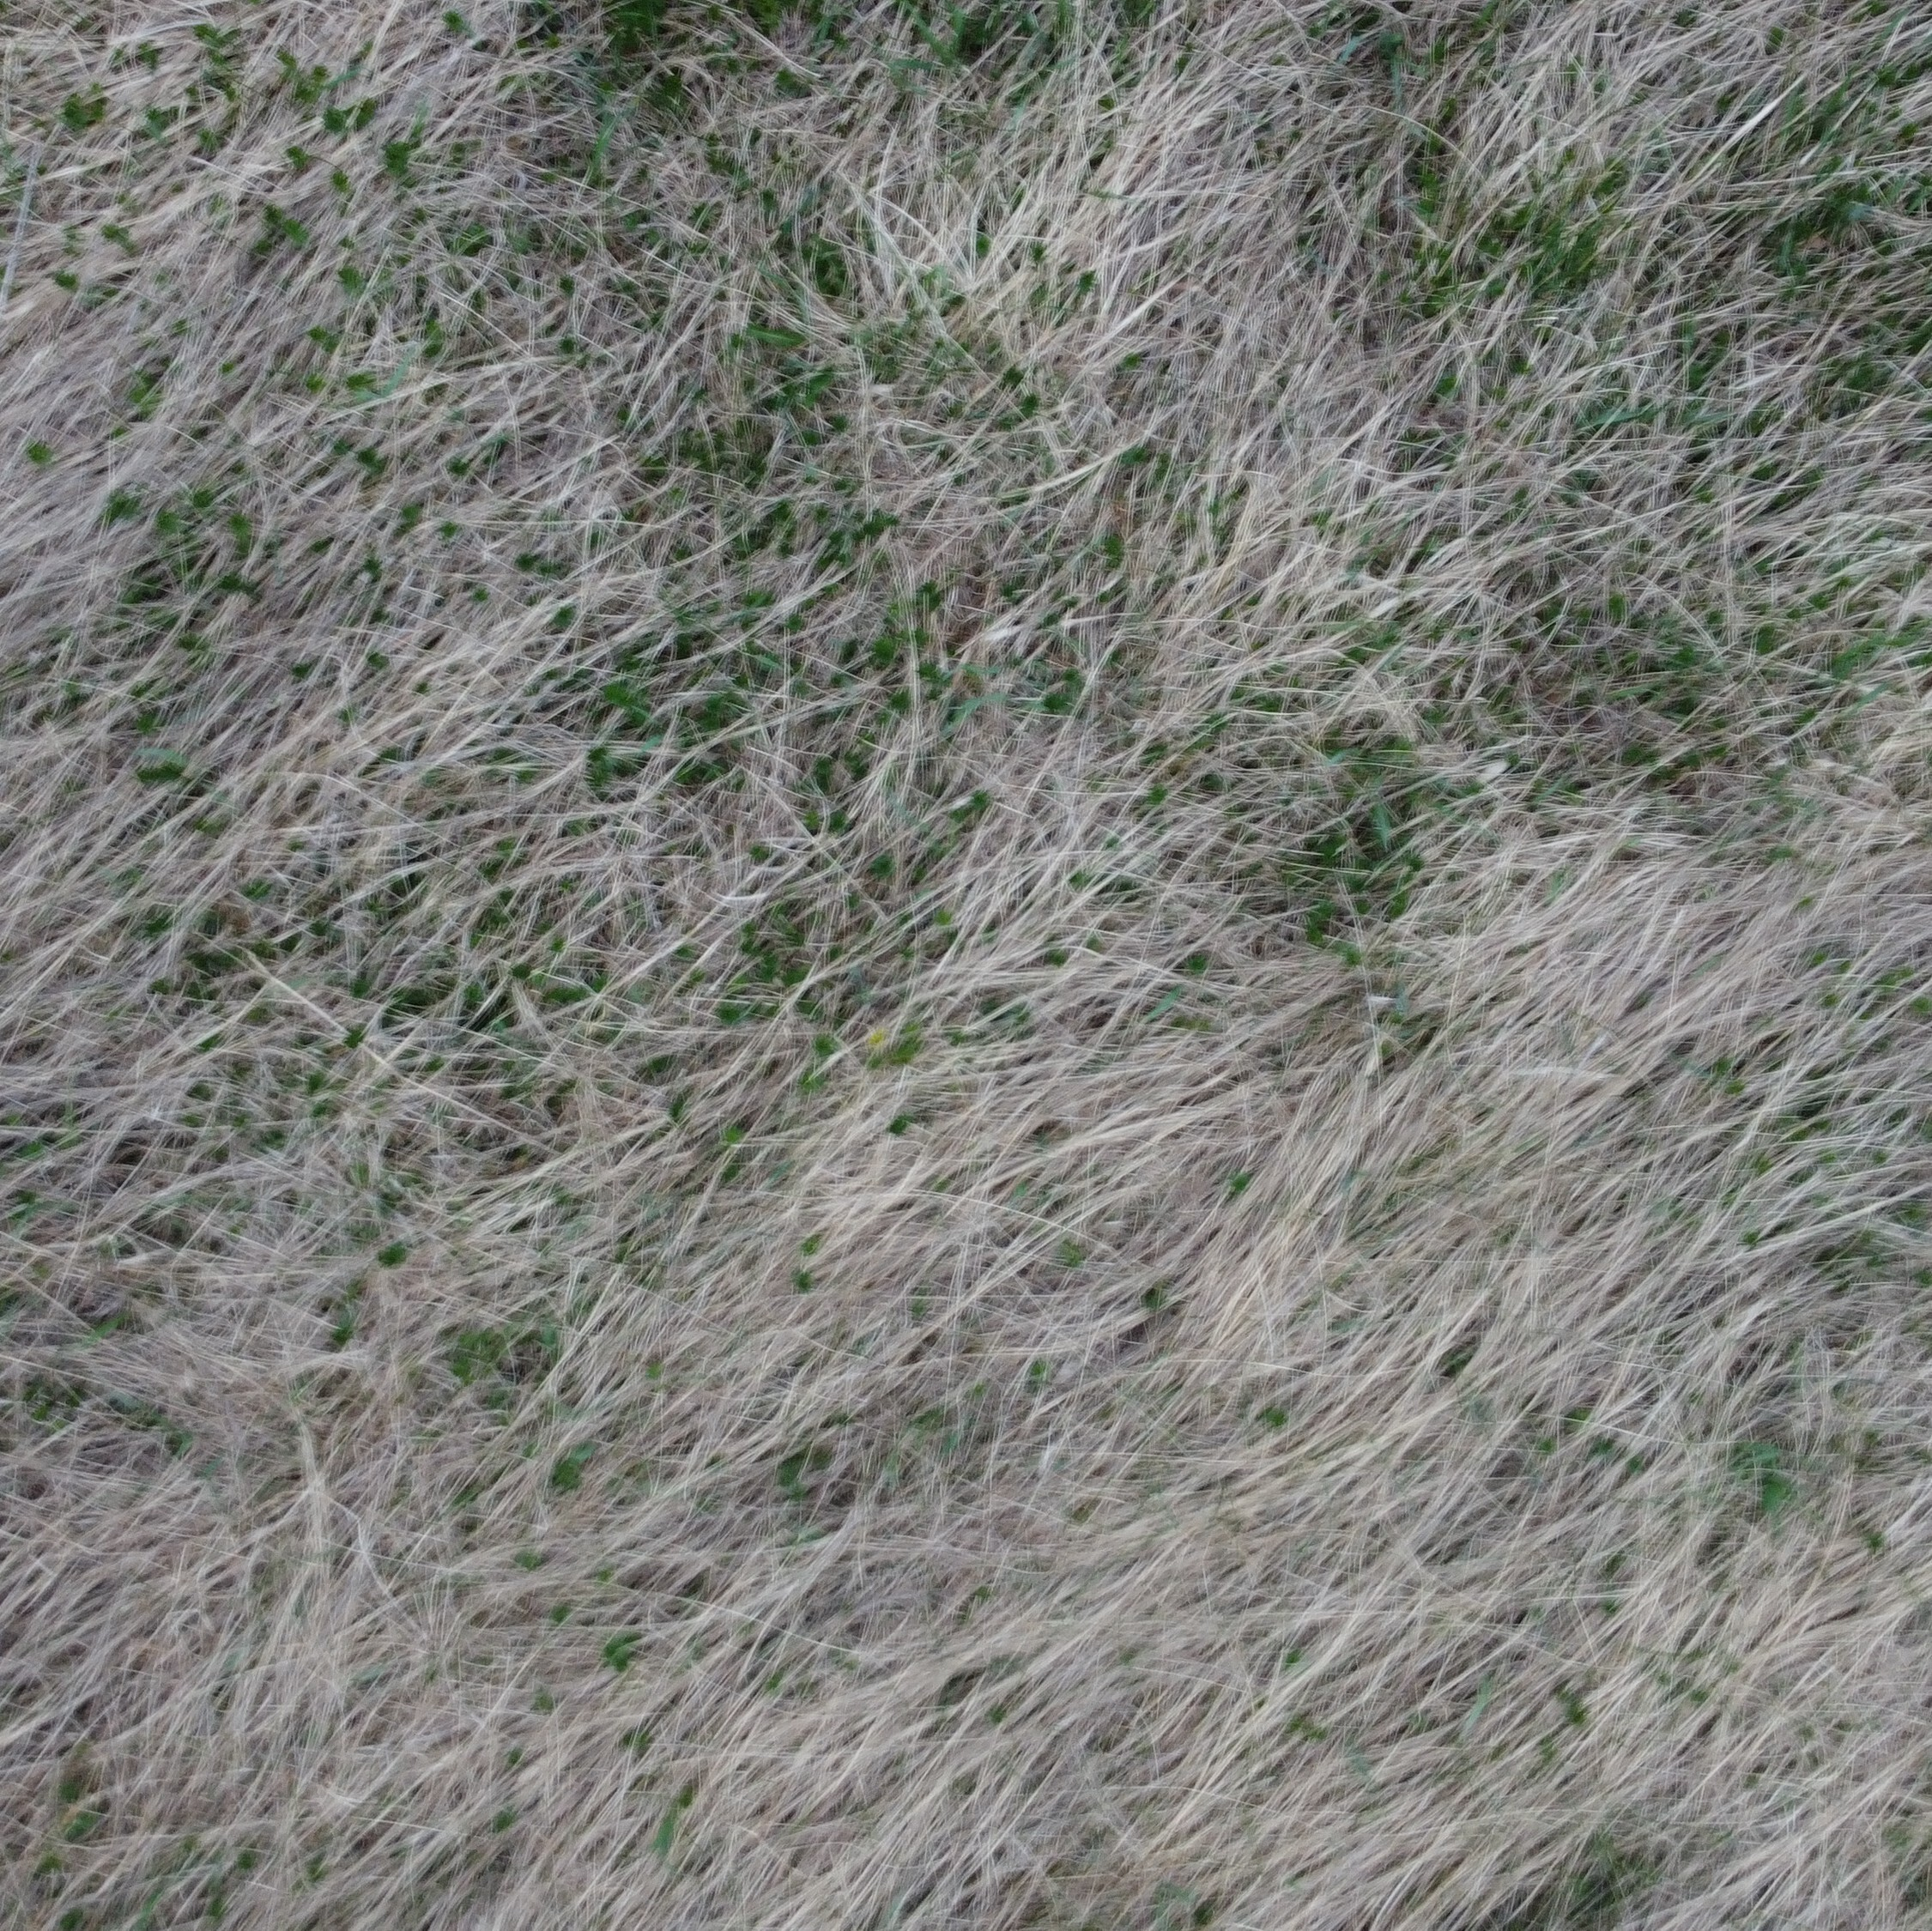
\includegraphics[width=0.7\linewidth,height=\textheight,keepaspectratio]{rot0/DJI_0362.JPG}

}

\subcaption{\label{fig-rawgrass}Raw Grass Image}

\end{minipage}%
%
\begin{minipage}[t]{0.50\linewidth}

\centering{

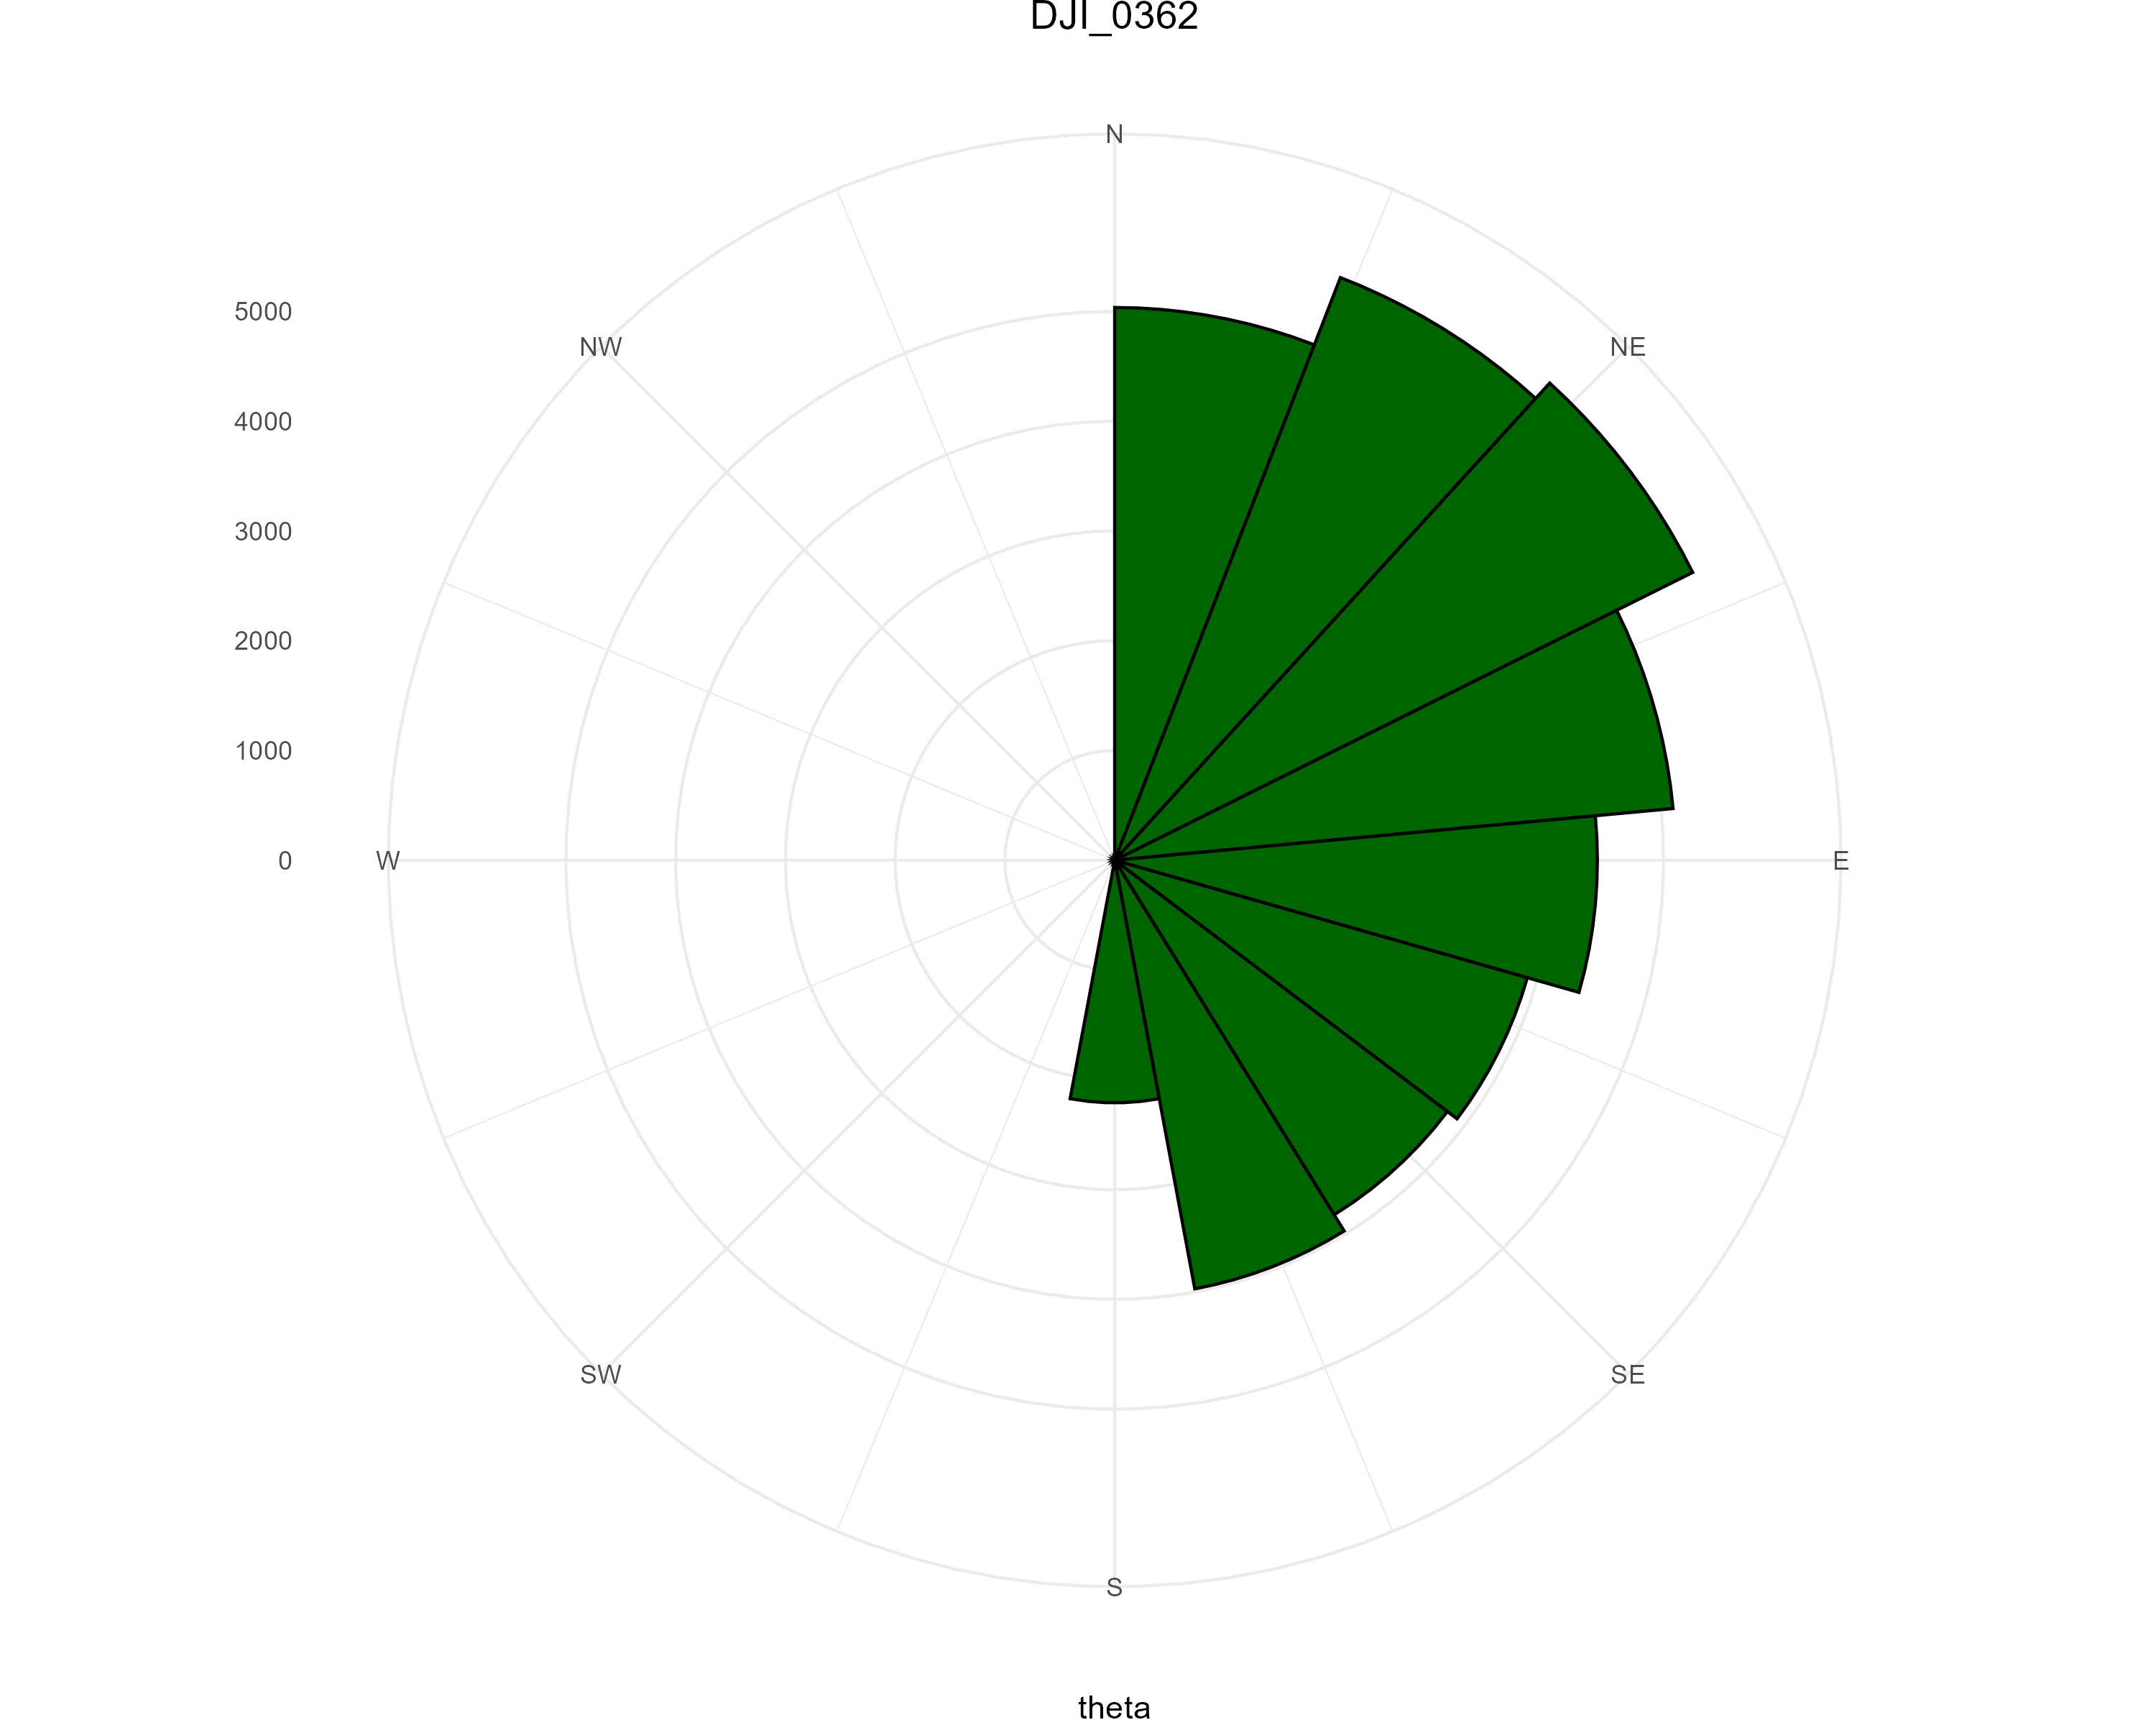
\includegraphics[width=0.95\linewidth,height=\textheight,keepaspectratio]{media/image_0362.png}

}

\subcaption{\label{fig-polarplot}Gradient Polar Plot}

\end{minipage}%

\caption{\label{fig-gradientplots}Gradient Analysis Polar Plot
Visualization.}

\end{figure}%

To summarize the pixel-level gradient angles extracted from each image,
weighted circular statistics are computed using the \texttt{tectonicr}
package in R. Because grass orientation is directional data that wraps
around, standard linear statistics such as a regular mean or variance
are not appropriate. Circular statistics are instead used, which account
for the nature of angular data. The gradient magnitude at each pixel
serves as a weight, meaning pixels with stronger intensity changes
indicating more defined grass edges contribute more to the overall
directional estimate than pixels in flat regions.

For each of the 65 images, four weighted circular statistics are
computed. The circular mean is the average dominant direction of
gradient angles across all pixels, weighted by magnitude, and represents
the algorithm's estimate of the overall grass lay direction in the
image. The circular variance measures how spread out the angles are
around this mean, where a value close to 0 indicates most pixels agree
on a similar direction and a value close to 1 indicates that there
directions of grass in the image are more varied. The circular median is
the central angle value that divides the weighted distribution in half.
The circular IQR measures the spread of the middle 50\% of the weighted
angle distribution, capturing variability in the dominant direction
without being influenced by extreme values.

\begin{Shaded}
\begin{Highlighting}[]
\CommentTok{\# Compute weighted circular statistics}
\NormalTok{  mean\_val }\OtherTok{\textless{}{-}} \FunctionTok{circular\_mean}\NormalTok{(angles, }\AttributeTok{w =}\NormalTok{ magnitudes, }\AttributeTok{axial =} \ConstantTok{TRUE}\NormalTok{, }\AttributeTok{na.rm =} \ConstantTok{TRUE}\NormalTok{)}
\NormalTok{  var\_val }\OtherTok{\textless{}{-}} \FunctionTok{circular\_var}\NormalTok{(angles, }\AttributeTok{w =}\NormalTok{ magnitudes, }\AttributeTok{axial =} \ConstantTok{TRUE}\NormalTok{, }\AttributeTok{na.rm =} \ConstantTok{TRUE}\NormalTok{)}
\NormalTok{  median\_val }\OtherTok{\textless{}{-}} \FunctionTok{circular\_median}\NormalTok{(angles, }\AttributeTok{w =}\NormalTok{ magnitudes, }\AttributeTok{axial =} \ConstantTok{TRUE}\NormalTok{, }\AttributeTok{na.rm =} \ConstantTok{TRUE}\NormalTok{)}
\NormalTok{  iqr\_val }\OtherTok{\textless{}{-}} \FunctionTok{circular\_IQR}\NormalTok{(angles, }\AttributeTok{w =}\NormalTok{ magnitudes, }\AttributeTok{axial =} \ConstantTok{TRUE}\NormalTok{, }\AttributeTok{na.rm =} \ConstantTok{TRUE}\NormalTok{)}
\NormalTok{  quantiles }\OtherTok{\textless{}{-}} \FunctionTok{circular\_quantiles}\NormalTok{(angles, }\AttributeTok{w =}\NormalTok{ magnitudes, }\AttributeTok{axial =} \ConstantTok{TRUE}\NormalTok{, }\AttributeTok{na.rm =} \ConstantTok{TRUE}\NormalTok{)}
  
\end{Highlighting}
\end{Shaded}

The \texttt{axial\ =\ TRUE} argument is used throughout because as
discusses earlier, the grass orientation is axial, meaning pixel-level
angles map onto a 0°--180° range rather than a full 360° scale, since a
grass blade pointing at 10° is indistinguishable from one pointing at
190°. The circular statistics therefore operate on the same 0°--180°
scale as the extracted angles, ensuring consistency between the
pixel-level gradient computation and the image-level summary statistics.
These statistics are compiled into a data frame with one row per image,
containing the image name, date taken, and the four circular statistics,
producing a full dataset for further analysis.
Table~\ref{tbl-gradientstats} shows a sample of this dataset.

\begin{table}

\caption{\label{tbl-gradientstats}}

\centering{

\centering
\begin{tabular}[t]{>{\raggedright\arraybackslash}p{3.5cm}>{\raggedleft\arraybackslash}p{2cm}>{\raggedleft\arraybackslash}p{2.5cm}>{\raggedleft\arraybackslash}p{2.5cm}>{\raggedleft\arraybackslash}p{2cm}}
\toprule
Image & Circ. Mean & Circ. Variance & Circ. Median & Circ. IQR\\
\midrule
\cellcolor{gray!10}{DJI\_0256} & \cellcolor{gray!10}{29.86624} & \cellcolor{gray!10}{0.9433418} & \cellcolor{gray!10}{86.04090} & \cellcolor{gray!10}{87.48395}\\
DJI\_0344 & 55.83333 & 0.9337435 & 86.11589 & 87.35129\\
\cellcolor{gray!10}{DJI\_0345} & \cellcolor{gray!10}{44.43737} & \cellcolor{gray!10}{0.9225823} & \cellcolor{gray!10}{84.41378} & \cellcolor{gray!10}{89.36600}\\
DJI\_0346 & 47.72566 & 0.9125125 & 82.86430 & 89.01660\\
\cellcolor{gray!10}{DJI\_0347} & \cellcolor{gray!10}{65.90795} & \cellcolor{gray!10}{0.9411583} & \cellcolor{gray!10}{86.89895} & \cellcolor{gray!10}{86.13982}\\
\addlinespace
DJI\_0348 & 51.95467 & 0.9250089 & 84.87817 & 87.91640\\
\cellcolor{gray!10}{DJI\_0349} & \cellcolor{gray!10}{46.13757} & \cellcolor{gray!10}{0.8978368} & \cellcolor{gray!10}{82.29246} & \cellcolor{gray!10}{88.02058}\\
DJI\_0350 & 58.83998 & 0.9009255 & 83.29214 & 85.42393\\
\bottomrule
\end{tabular}

}

\end{table}%

To validate the gradient analysis results, human assessments of the same
65 SLU Living Lab images were collected using a custom R Shiny web
application, described in the following section.

\subsection{Human Assessment of Grass Lay Using R Shiny Web
App}\label{human-assessment-of-grass-lay-using-r-shiny-web-app}

As discussed earlier, the Traditional Ecological Knowledge (TEK) of
physically observing grass lay is a method used by Arctic community
members. Hunters and gatherers will observe the direction plants lay
down after the growing season as proxies for predominant wind direction
and wind direction change. To replicate this process conducted by
humans, we customized an app to retrieve volunteers' perceptions of
direction that grass lays. Shiny is an R package that makes it easy to
build interactive web applications straight from R (Posit (2026)). We
used Shiny to customize an interactive grass app to collect human
assessments of the grass images dominant grass lay direction. 45
volunteers completed the assessment of all 65 grass images. Each
participant session is assigned a unique \texttt{UUID} to ensure
anonymity while preserving response traceability. The application
presents users with the series of grass images and prompts them to
indicate the dominant direction of grass lay by clicking directly on the
image. Upon clicking, a visual arrow is displayed to reflect the
selected direction, allowing users to adjust their response before
submission. See Figure~\ref{fig-grassapp}.

\begin{figure}[H]

\centering{

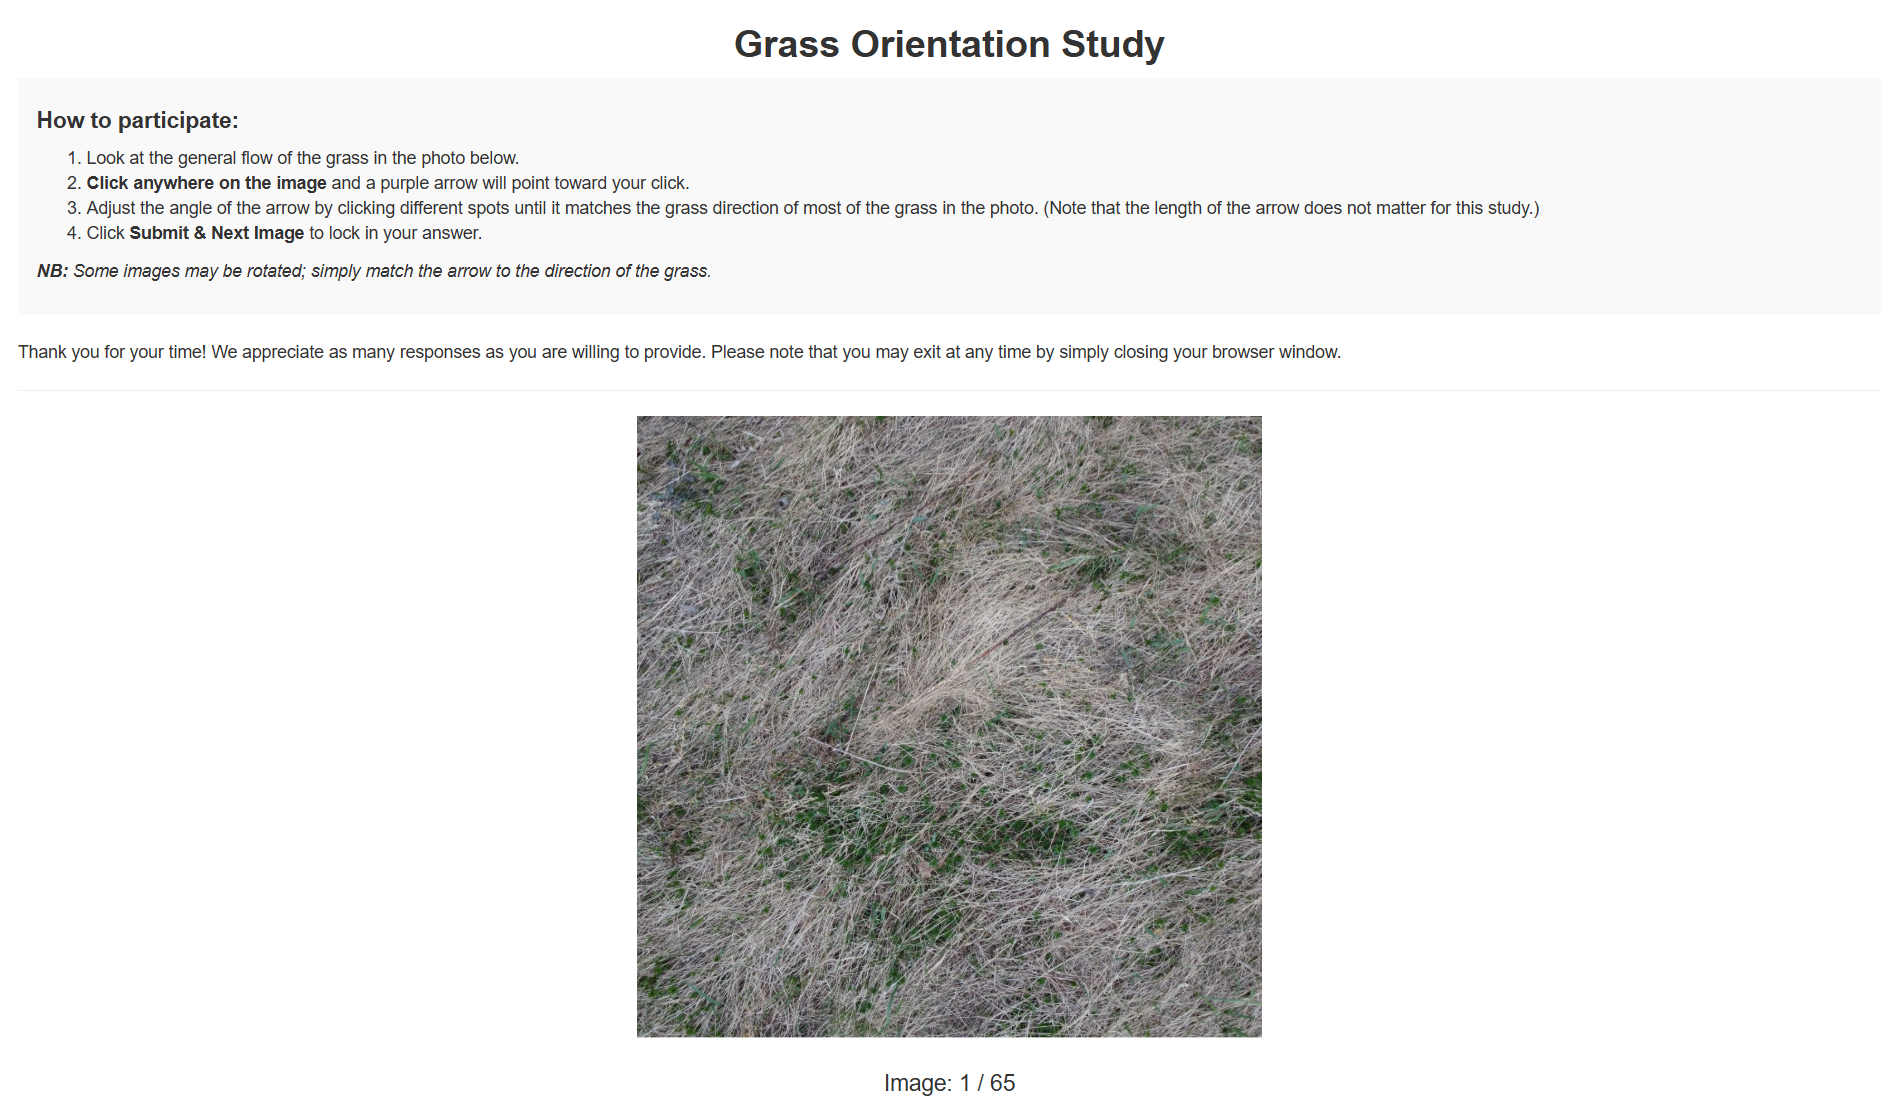
\includegraphics[width=1\linewidth,height=\textheight,keepaspectratio]{media/grassapp.png}

}

\caption{\label{fig-grassapp}\href{https://franmnenula.shinyapps.io/grassapp_v1/}{Custom
Shiny Grass App}}

\end{figure}%

The 65 grass images are stored in a GitHub repository and retrieved at
the start of each session using the GitHub API. The API call constructs
a URL pointing to the images folder of the repository and uses
\texttt{jsonlite::fromJSON()} to parse the response, extracting all
filenames with image extensions into a master list called
\texttt{img\_master\_global}. This approach avoids hardcoding file paths
and ensures the full image set is always current without needing to
update the app code when images change.

\begin{Shaded}
\begin{Highlighting}[]
\CommentTok{\# Github variables}
\NormalTok{repo\_owner }\OtherTok{\textless{}{-}} \StringTok{"franriee"}
\NormalTok{repo\_name }\OtherTok{\textless{}{-}} \StringTok{"SYE\_Grass\_Study"}

\CommentTok{\# Use regular images folder to get the master list of filenames}
\NormalTok{folder\_api }\OtherTok{\textless{}{-}} \FunctionTok{paste0}\NormalTok{(}\StringTok{"https://api.github.com/repos/"}\NormalTok{, }
\NormalTok{repo\_owner, }\StringTok{"/"}\NormalTok{, repo\_name, }\StringTok{"/contents/images"}\NormalTok{)}
\NormalTok{files }\OtherTok{\textless{}{-}}\NormalTok{ jsonlite}\SpecialCharTok{::}\FunctionTok{fromJSON}\NormalTok{(folder\_api)}

\CommentTok{\# Create a data frame to keep the image names }
\NormalTok{img\_master\_global }\OtherTok{\textless{}{-}} \FunctionTok{data.frame}\NormalTok{(}
  \AttributeTok{name =}\NormalTok{ files}\SpecialCharTok{$}\NormalTok{name[}\FunctionTok{grepl}\NormalTok{(}\StringTok{"}\SpecialCharTok{\textbackslash{}\textbackslash{}}\StringTok{.(png|jpg|jpeg)$"}\NormalTok{, files}\SpecialCharTok{$}\NormalTok{name, }
  \AttributeTok{ignore.case =} \ConstantTok{TRUE}\NormalTok{)], }
  \AttributeTok{stringsAsFactors =} \ConstantTok{FALSE}
\NormalTok{)}
\end{Highlighting}
\end{Shaded}

When a new participant session begins, the Shiny server creates a
session-specific shuffled copy of \texttt{img\_master\_global} by
randomly reordering the rows using \texttt{sample()}. This means every
participant sees the same 65 images but in a different order, reducing
ordering effects where earlier images might systematically influence
responses to later ones. To further reduce bias, a random rotation is
pre-assigned to every image for that session by sampling from 0°, 90°,
180°, and 270°. This is important because the region the St.~Lawrence
University Living Laboratory is located experiences predominant
northeasterly winds, and volunteers familiar with the site may already
know this. Without rotation, a participant who recognizes the field's
geographic orientation could use that prior knowledge to guess that
grass lays in the direction of the prevailing northeast wind rather than
genuinely assessing the direction they perceive from the image itself.
By randomly rotating each image before display, no fixed compass
orientation is preserved, ensuring that responses reflect the
participant's actual visual perception of grass lay direction rather
than recalled knowledge of local wind patterns.

\begin{Shaded}
\begin{Highlighting}[]
\NormalTok{server }\OtherTok{\textless{}{-}} \ControlFlowTok{function}\NormalTok{(input, output, session) \{}
\NormalTok{  img\_master }\OtherTok{\textless{}{-}}\NormalTok{ img\_master\_global[}\FunctionTok{sample}\NormalTok{(}\FunctionTok{nrow}\NormalTok{(img\_master\_global)), }
\NormalTok{  , drop }\OtherTok{=} \ConstantTok{FALSE}\NormalTok{]}
  
\NormalTok{  session\_rotations }\OtherTok{\textless{}{-}} \FunctionTok{sample}\NormalTok{(}\FunctionTok{c}\NormalTok{(}\DecValTok{0}\NormalTok{, }\DecValTok{90}\NormalTok{, }\DecValTok{180}\NormalTok{, }\DecValTok{270}\NormalTok{), }
  \FunctionTok{nrow}\NormalTok{(img\_master), }\AttributeTok{replace =} \ConstantTok{TRUE}\NormalTok{)}
\end{Highlighting}
\end{Shaded}

Each image is displayed using a Plotly-based interface. \texttt{Plotly}
is an interactive graphing library in R that supports event-driven
interactions such as mouse clicks, making it well suited for collecting
user input directly on top of an image (Plotly Technologies Inc.
(2026)). The image is overlaid onto a coordinate grid ranging from 0 to
1 in both the x and y dimensions, rendered as a background layer beneath
an invisible heatmap. This design allows click positions to be precisely
recorded without needing to re-render the grass image each time the
participant adjusts their arrow.

\begin{Shaded}
\begin{Highlighting}[]
\FunctionTok{plot\_ly}\NormalTok{(}
      \AttributeTok{x =}\NormalTok{ g, }\AttributeTok{y =}\NormalTok{ g, }\AttributeTok{z =}\NormalTok{ z,}
      \AttributeTok{type =} \StringTok{"heatmap"}\NormalTok{,}
      \AttributeTok{showscale =} \ConstantTok{FALSE}\NormalTok{,}
      \AttributeTok{hoverinfo =} \StringTok{"none"}\NormalTok{,}
      \AttributeTok{source =} \StringTok{"grass\_plot"}\NormalTok{,}
      \AttributeTok{colorscale =} \FunctionTok{list}\NormalTok{(}\FunctionTok{list}\NormalTok{(}\DecValTok{0}\NormalTok{, }\StringTok{"rgba(0,0,0,0)"}\NormalTok{), }
      \FunctionTok{list}\NormalTok{(}\DecValTok{1}\NormalTok{, }\StringTok{"rgba(0,0,0,0)"}\NormalTok{))}
\NormalTok{    ) }\SpecialCharTok{\%\textgreater{}\%}
      \FunctionTok{layout}\NormalTok{(}
        \AttributeTok{xaxis =} \FunctionTok{list}\NormalTok{(}\AttributeTok{range =} \FunctionTok{c}\NormalTok{(}\DecValTok{0}\NormalTok{, }\DecValTok{1}\NormalTok{), }\AttributeTok{visible =} \ConstantTok{FALSE}\NormalTok{, }
        \AttributeTok{fixedrange =} \ConstantTok{TRUE}\NormalTok{),}
        \AttributeTok{yaxis =} \FunctionTok{list}\NormalTok{(}\AttributeTok{range =} \FunctionTok{c}\NormalTok{(}\DecValTok{0}\NormalTok{, }\DecValTok{1}\NormalTok{), }\AttributeTok{visible =} \ConstantTok{FALSE}\NormalTok{, }
        \AttributeTok{fixedrange =} \ConstantTok{TRUE}\NormalTok{, }\AttributeTok{scaleanchor =} \StringTok{"x"}\NormalTok{),}
        \AttributeTok{images =} \FunctionTok{list}\NormalTok{(}\FunctionTok{list}\NormalTok{(}
          \AttributeTok{source =}\NormalTok{ github\_raw\_url,}
          \AttributeTok{x =} \DecValTok{0}\NormalTok{, }\AttributeTok{y =} \DecValTok{1}\NormalTok{, }\AttributeTok{sizex =} \DecValTok{1}\NormalTok{, }\AttributeTok{sizey =} \DecValTok{1}\NormalTok{,}
          \AttributeTok{xref =} \StringTok{"x"}\NormalTok{, }\AttributeTok{yref =} \StringTok{"y"}\NormalTok{, }\AttributeTok{sizing =} \StringTok{"contain"}\NormalTok{, }
          \AttributeTok{layer =} \StringTok{"below"}
\NormalTok{        )),}
        \AttributeTok{margin =} \FunctionTok{list}\NormalTok{(}\AttributeTok{l=}\DecValTok{0}\NormalTok{, }\AttributeTok{r=}\DecValTok{0}\NormalTok{, }\AttributeTok{t=}\DecValTok{0}\NormalTok{, }\AttributeTok{b=}\DecValTok{0}\NormalTok{),}
        \AttributeTok{annotations =} \FunctionTok{list}\NormalTok{() }\CommentTok{\# Clear old arrows on re{-}render}
\NormalTok{      ) }\SpecialCharTok{\%\textgreater{}\%}
      \FunctionTok{config}\NormalTok{(}\AttributeTok{displayModeBar =} \ConstantTok{FALSE}\NormalTok{)}
  \ErrorTok{\})}
\end{Highlighting}
\end{Shaded}

When a participant clicks on the image, Plotly captures the click
coordinates \texttt{d\$x} and \texttt{d\$y}. The angular direction of
the click is then computed relative to the center of the image at
\texttt{(0.5,\ 0.5)}. The horizontal and vertical distances from the
center, \texttt{dx} and \texttt{dy}, are passed to \texttt{atan2()}
which computes the angle in radians and converts it to degrees. The
result is mapped onto a 0°--360° circular scale using the modulo
operator \texttt{\%\%\ 360}. A visual arrow is then rendered from the
image center to the click position using \texttt{plotlyProxyInvoke()},
which updates only the annotation layer of the plot without re-rendering
the background image, allowing the participant to adjust their response
smoothly before submitting.

\begin{Shaded}
\begin{Highlighting}[]
  \CommentTok{\# Listen for plotly click}
  \FunctionTok{observeEvent}\NormalTok{(}\FunctionTok{event\_data}\NormalTok{(}\StringTok{"plotly\_click"}\NormalTok{, }\AttributeTok{source =} \StringTok{"grass\_plot"}\NormalTok{), }
\NormalTok{  \{ }
\NormalTok{    d }\OtherTok{\textless{}{-}} \FunctionTok{event\_data}\NormalTok{(}\StringTok{"plotly\_click"}\NormalTok{, }\AttributeTok{source =} \StringTok{"grass\_plot"}\NormalTok{)}
    \FunctionTok{req}\NormalTok{(d) }\CommentTok{\# require that the click is not null}
    
    \CommentTok{\# Update the last saved clicks}
    \FunctionTok{last\_click\_x}\NormalTok{(d}\SpecialCharTok{$}\NormalTok{x)}
    \FunctionTok{last\_click\_y}\NormalTok{(d}\SpecialCharTok{$}\NormalTok{y)}
    
    \CommentTok{\# Angle calculation from center (0.5, 0.5)}
\NormalTok{    dx }\OtherTok{\textless{}{-}}\NormalTok{ d}\SpecialCharTok{$}\NormalTok{x }\SpecialCharTok{{-}} \FloatTok{0.5}
\NormalTok{    dy }\OtherTok{\textless{}{-}}\NormalTok{ d}\SpecialCharTok{$}\NormalTok{y }\SpecialCharTok{{-}} \FloatTok{0.5}
    
    \CommentTok{\# Convert x,y to degrees (using atan2)}
\NormalTok{    res\_angle }\OtherTok{\textless{}{-}}\NormalTok{ (}\FunctionTok{atan2}\NormalTok{(dx, dy) }\SpecialCharTok{*} \DecValTok{180} \SpecialCharTok{/}\NormalTok{ pi) }\SpecialCharTok{\%\%} \DecValTok{360}
    \FunctionTok{current\_angle}\NormalTok{(res\_angle)}
    
    \CommentTok{\# Update arrow}
    \CommentTok{\# plotlyProxy to modify only the annotation layer of the plot}
    \CommentTok{\# relayout updates the arrow position instantly without }
    \CommentTok{\# re{-}rendering the background grass image}
    \FunctionTok{plotlyProxy}\NormalTok{(}\StringTok{"img\_display"}\NormalTok{, session) }\SpecialCharTok{\%\textgreater{}\%}
      \FunctionTok{plotlyProxyInvoke}\NormalTok{(}\StringTok{"relayout"}\NormalTok{, }\FunctionTok{list}\NormalTok{(}
        \AttributeTok{annotations =} \FunctionTok{list}\NormalTok{(}\FunctionTok{list}\NormalTok{(}
          \AttributeTok{x =}\NormalTok{ d}\SpecialCharTok{$}\NormalTok{x, }\AttributeTok{y =}\NormalTok{ d}\SpecialCharTok{$}\NormalTok{y,}
          \AttributeTok{ax =} \FloatTok{0.5}\NormalTok{, }\AttributeTok{ay =} \FloatTok{0.5}\NormalTok{,}
          \AttributeTok{xref =} \StringTok{"x"}\NormalTok{, }\AttributeTok{yref =} \StringTok{"y"}\NormalTok{,}
          \AttributeTok{axref =} \StringTok{"x"}\NormalTok{, }\AttributeTok{ayref =} \StringTok{"y"}\NormalTok{,}
          \AttributeTok{text =} \StringTok{""}\NormalTok{, }
          \AttributeTok{showarrow =} \ConstantTok{TRUE}\NormalTok{,}
          \AttributeTok{arrowwidth =} \DecValTok{5}\NormalTok{,}
          \AttributeTok{arrowhead =} \DecValTok{3}\NormalTok{,}
          \AttributeTok{arrowcolor =} \StringTok{"\#4B0082"}
\NormalTok{        ))}
\NormalTok{      ))}
\NormalTok{  \})}
\ErrorTok{\}}
\end{Highlighting}
\end{Shaded}

In addition to the angular direction, the Euclidean distance from the
image center to the click position is recorded as a magnitude value,
computed from \texttt{dx} and \texttt{dy} using the Pythagorean formula.
This distance serves as a proxy for response confidence where a click
far from the center suggests a more deliberate directional choice, while
a click at or very close to the center may indicate uncertainty in their
choice of dominant grass lay. Because the arrow defaults to the center
position \texttt{(0.5,\ 0.5)} before any click is made, a magnitude of 0
means the participant submitted without clicking, leaving the angle
unchanged from its default value. We assume that these submissions do
not represent a genuine assessment of grass direction and would
introduce noise into the circular statistics. To address this, responses
with a magnitude of exactly 0 were filtered out before computing the
per-image circular statistics, retaining only submissions where the
participant made a deliberate click away from the center.

\begin{Shaded}
\begin{Highlighting}[]
 \CommentTok{\# Get the click}
\NormalTok{    cx }\OtherTok{\textless{}{-}} \FunctionTok{last\_click\_x}\NormalTok{()}
\NormalTok{    cy }\OtherTok{\textless{}{-}} \FunctionTok{last\_click\_y}\NormalTok{()}
\NormalTok{    dx }\OtherTok{\textless{}{-}}\NormalTok{ cx }\SpecialCharTok{{-}} \FloatTok{0.5}
\NormalTok{    dy }\OtherTok{\textless{}{-}}\NormalTok{ cy }\SpecialCharTok{{-}} \FloatTok{0.5}
\NormalTok{    mag }\OtherTok{\textless{}{-}} \FunctionTok{sqrt}\NormalTok{(dx}\SpecialCharTok{\^{}}\DecValTok{2} \SpecialCharTok{+}\NormalTok{ dy}\SpecialCharTok{\^{}}\DecValTok{2}\NormalTok{)}
\end{Highlighting}
\end{Shaded}

All responses are stored in real time using the Google Sheets API via
the \texttt{googlesheets4} package, enabling immediate cloud-based
logging into a Google Sheet without local storage dependencies. After
each submission, a row is appended to the connected Google Sheet
containing the participant's unique session ID, the image name, the
displayed rotation, the raw submitted angle, the true angle corrected
for rotation by reversing the applied rotation
\texttt{(current\_angle()\ -\ rotation()\ \%\%\ 360)}, the click
coordinates, the magnitude, and a timestamp. This structure ensures full
reproducibility and traceability of all responses.

\begin{Shaded}
\begin{Highlighting}[]
\CommentTok{\# Google sheets connection}
\FunctionTok{gs4\_auth}\NormalTok{(}\AttributeTok{path =} \StringTok{"xxxxxxx.json"}\NormalTok{)}
\NormalTok{sheet\_url }\OtherTok{\textless{}{-}} \StringTok{"https://xxxxxxxxxxx"}
\NormalTok{codes\_sheet\_url }\OtherTok{\textless{}{-}} \StringTok{"https://xxxxxxxx"}

\CommentTok{\# Add to Google Sheet}
    \CommentTok{\# Upon submission, create the row of data by creating a df}
    \CommentTok{\# Retrieve the name of the image the user is seeing}
    \CommentTok{\# Add the new data to the Google Sheet (sheet)}
    \FunctionTok{sheet\_append}\NormalTok{(sheet\_url, }\FunctionTok{data.frame}\NormalTok{(}
      \AttributeTok{UserID =}\NormalTok{ user\_session\_id,}
      \AttributeTok{Image =}\NormalTok{ img\_master}\SpecialCharTok{$}\NormalTok{name[}\FunctionTok{idx}\NormalTok{()], }
      \AttributeTok{User\_Angle =} \FunctionTok{round}\NormalTok{(}\FunctionTok{current\_angle}\NormalTok{(), }\DecValTok{2}\NormalTok{),}
      \AttributeTok{True\_Angle =} \FunctionTok{round}\NormalTok{((}\FunctionTok{current\_angle}\NormalTok{() }\SpecialCharTok{{-}} \FunctionTok{rotation}\NormalTok{()) }\SpecialCharTok{\%\%} \DecValTok{360}\NormalTok{, }
      \DecValTok{2}\NormalTok{), }\CommentTok{\# reverse the rotation and that is the true angle}
      \AttributeTok{Rotation =} \FunctionTok{rotation}\NormalTok{(),}
      \AttributeTok{Timestamp =} \FunctionTok{format}\NormalTok{(}\FunctionTok{Sys.time}\NormalTok{(), }\AttributeTok{tz =} \StringTok{"America/New\_York"}\NormalTok{),}
      \AttributeTok{Coord\_x =} \FunctionTok{round}\NormalTok{(cx, }\DecValTok{4}\NormalTok{),}
      \AttributeTok{Coord\_y =} \FunctionTok{round}\NormalTok{(cy, }\DecValTok{4}\NormalTok{),}
      \AttributeTok{Magnitude =} \FunctionTok{round}\NormalTok{(mag, }\DecValTok{2}\NormalTok{)}
\NormalTok{    ), }\AttributeTok{sheet =} \StringTok{"Results"}\NormalTok{)}
\end{Highlighting}
\end{Shaded}

Just as with the gradient analysis, the submitted human responses are
summarized using circular statistics including circular mean, variance,
median, and interquartile range that are computed per image across all
45 participants. This produces a data frame of one row per image
containing the human assessment circular statistics, which is then
compared directly against the gradient analysis results to evaluate how
closely the algorithm's dominant direction estimate matches human
perception.

The findings from both the gradient analysis techniques and the human
assessment of images were compared to evaluate the validity of results
obtained from the gradient analysis techniques. The next section will
highlight the results as well as assess this data's association with
wind data during the growing season the previous year.

\clearpage

\section{Results}\label{results}

\subsection{Compare Results Between Gradient Analysis and Human
Assessment}\label{compare-results-between-gradient-analysis-and-human-assessment}

To evaluate the differences between the results from the Gradient
Analysis and Human Assessment, we computed the circular distances
between the two methods' circular means that is the dominant direction
of grass estimated from each image using both techniques. Circular
distance is used rather than a simple numerical difference because grass
orientation is axial data, meaning the difference between two angles
must account for the circular nature of the data. The
\texttt{circular\_distance()} function from the \texttt{tectonicr}
package computes this, returning values on a scale of 0 to 1, where 0
means the two methods agree perfectly on the same direction and 1 means
they are as far apart as possible which would mean pointing in
completely opposite directions measured in degrees.

\begin{Shaded}
\begin{Highlighting}[]
\CommentTok{\# Calculate distances between human vs hog}
\NormalTok{diff\_df }\OtherTok{\textless{}{-}} \FunctionTok{data.frame}\NormalTok{(}
  \AttributeTok{image =}\NormalTok{ hog\_df}\SpecialCharTok{$}\NormalTok{image\_name,}
  \AttributeTok{human\_angle =}\NormalTok{ human\_df}\SpecialCharTok{$}\NormalTok{circular\_mean,}
  \AttributeTok{hog\_angle =}\NormalTok{ hog\_df}\SpecialCharTok{$}\NormalTok{circular\_mean,}
  \AttributeTok{circular\_distance =} \FunctionTok{circular\_distance}\NormalTok{(human\_df}\SpecialCharTok{$}\NormalTok{circular\_mean,}
\NormalTok{  hog\_df}\SpecialCharTok{$}\NormalTok{circular\_mean, }\AttributeTok{axial =} \ConstantTok{TRUE}\NormalTok{, }\AttributeTok{na.rm =} \ConstantTok{TRUE}\NormalTok{))}

\NormalTok{diff\_df}

\FunctionTok{write\_csv}\NormalTok{(diff\_df, }\FunctionTok{file.path}\NormalTok{(output\_dir, }\StringTok{"diff\_df.csv"}\NormalTok{))}
\end{Highlighting}
\end{Shaded}

To help calibrate what these values mean in practice: a circular
distance of 0 indicates perfect agreement, 0.25 corresponds to a
moderate directional difference of roughly 22.5°, 0.5 corresponds to a
45° difference, and 1.0 is the maximum possible.

The mean circular distance across all 65 images is 0.26 with a variance
of 0.09, suggesting that on average the gradient analysis and human
assessment are in moderate agreement on average. The minimum circular
distance of 0.0006 indicates near-perfect agreement for at least one
image, while the maximum of 0.999 indicates that for at least one image
the two methods produced nearly perpendicular dominant direction
estimates. There are a number of images where both methods closely
align, but also a number where they diverge substantially. In
Figure~\ref{fig-results}, the yellow arrow represents the dominant
direction estimated by the gradient analysis and the black arrow
represents the human assessment, illustrating examples of both low,
medium, and high circular distance cases.

\begin{figure}[H]

\begin{minipage}[t]{0.33\linewidth}

\centering{

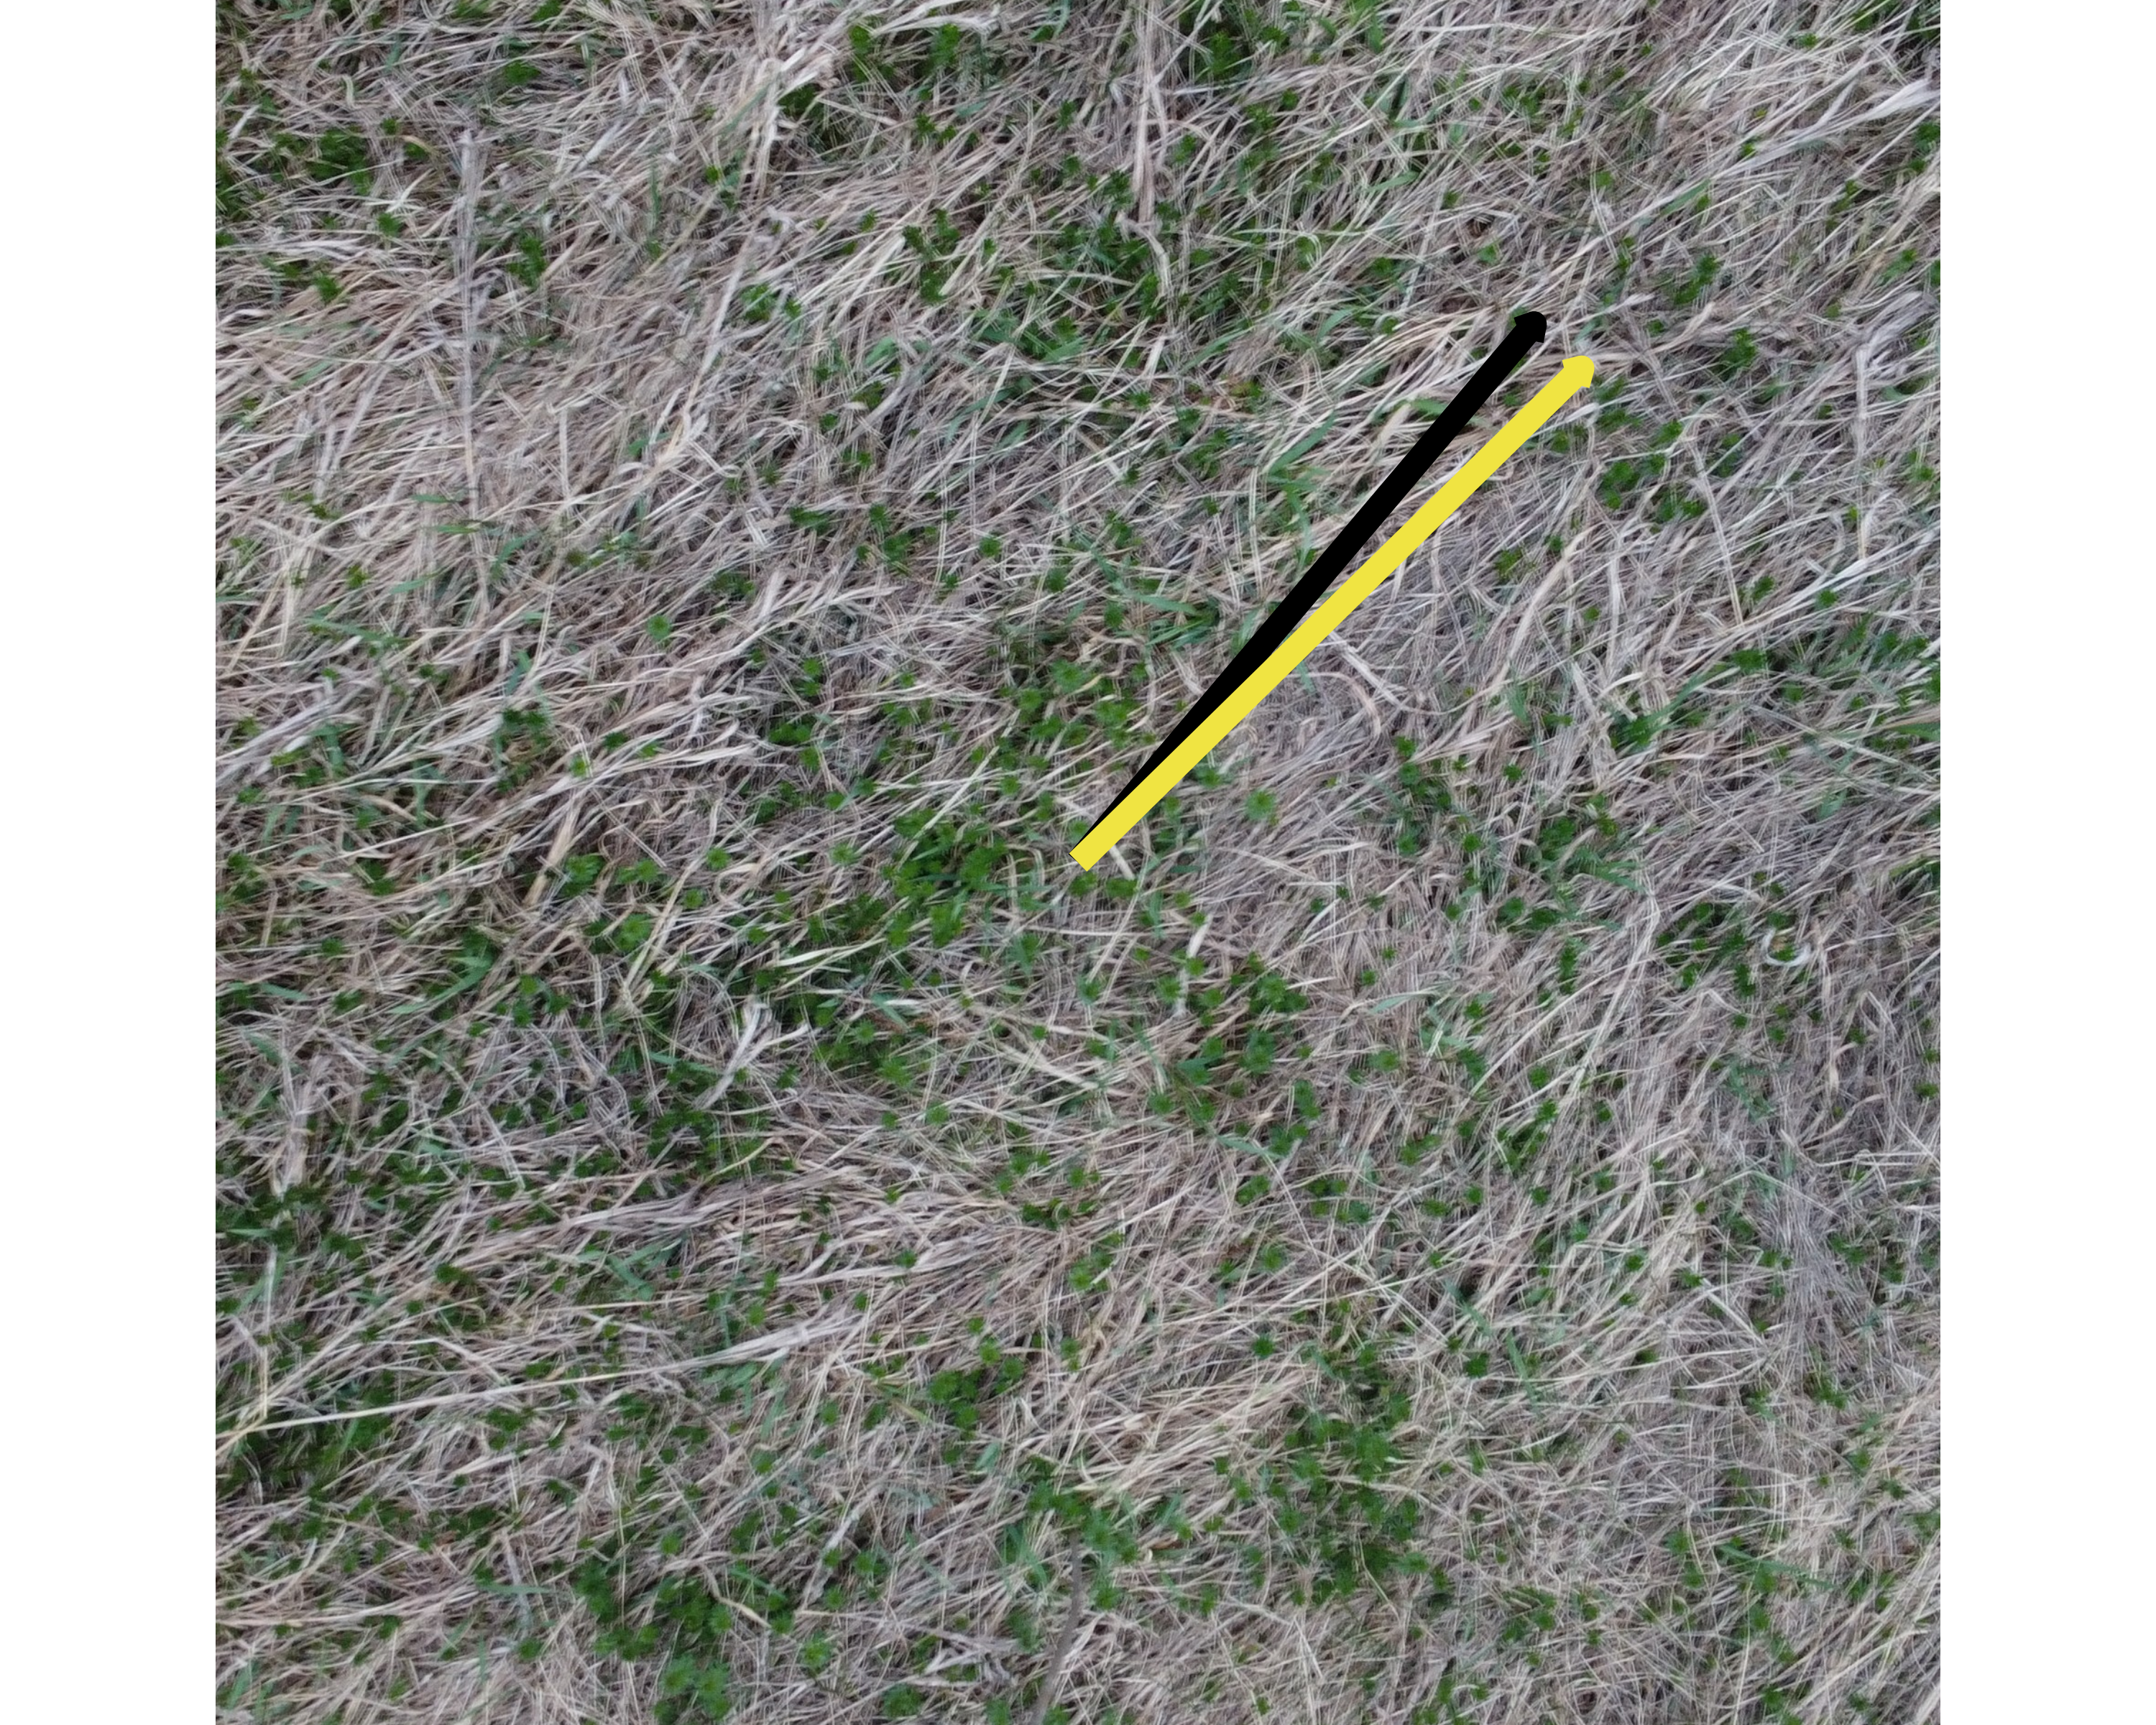
\includegraphics[width=0.8\linewidth,height=\textheight,keepaspectratio]{media/minimages.png}

}

\subcaption{\label{fig-resultmin}Low = 0.0084}

\end{minipage}%
%
\begin{minipage}[t]{0.33\linewidth}

\centering{

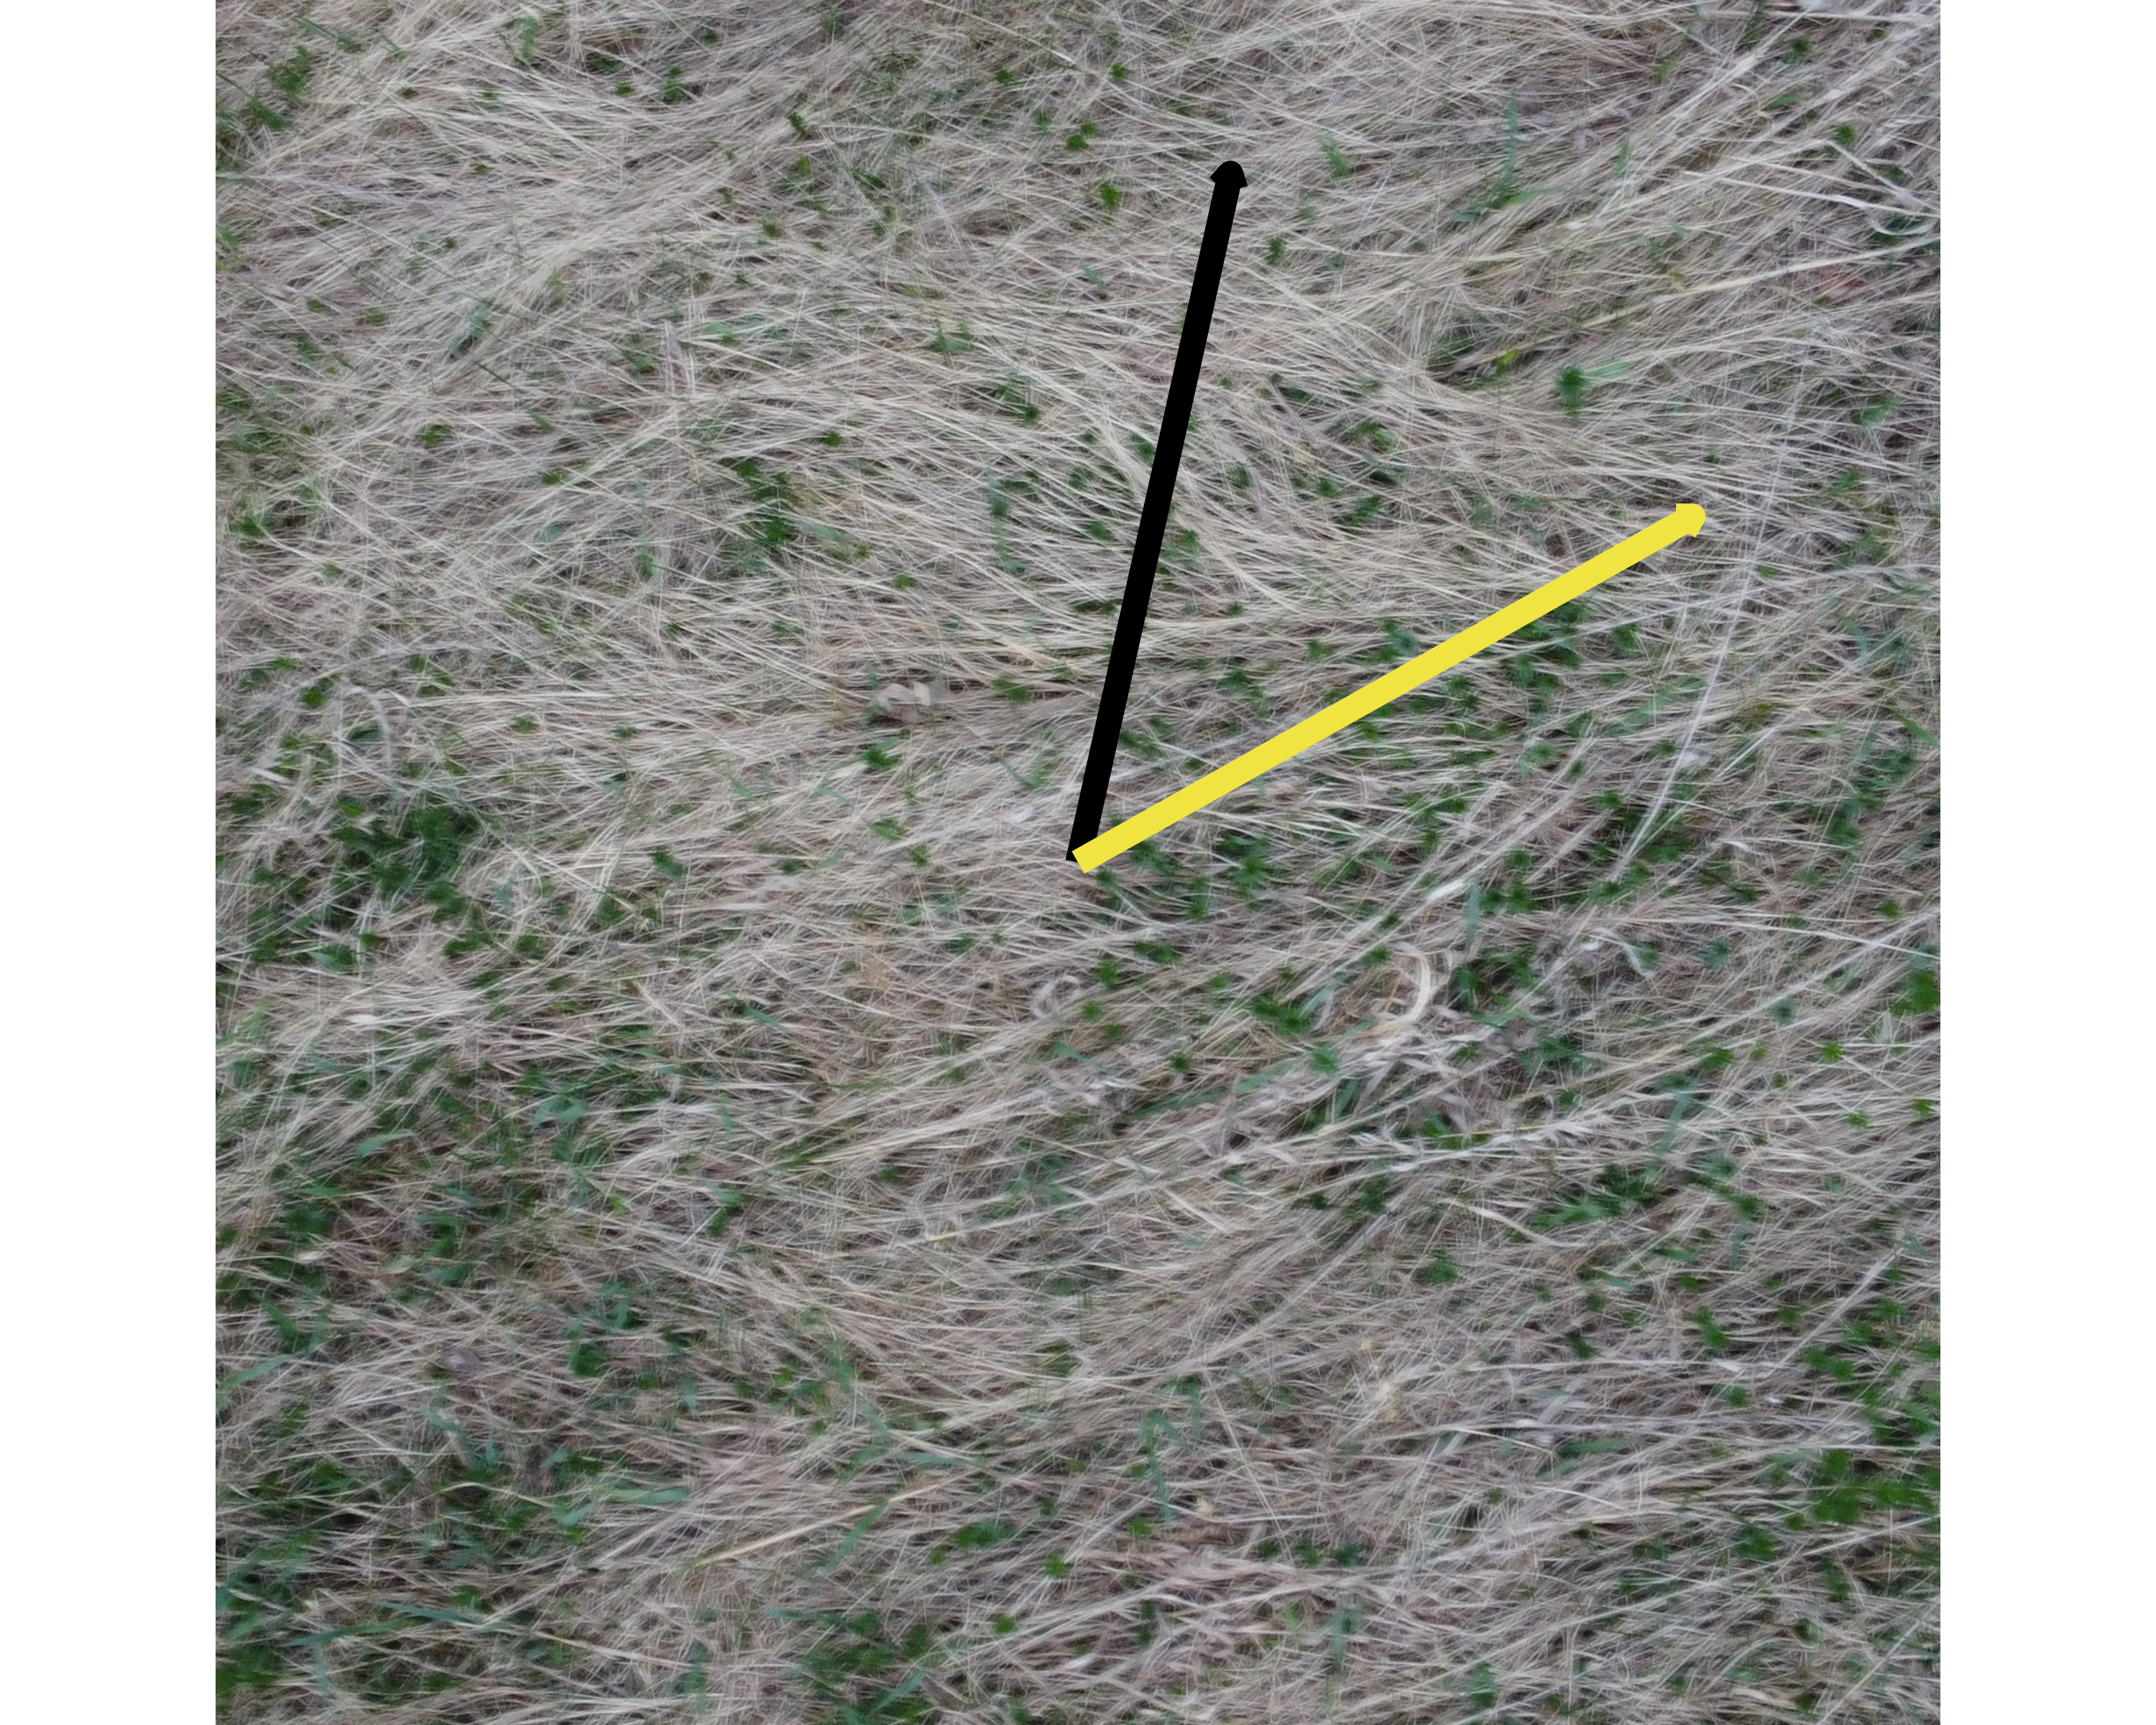
\includegraphics[width=0.8\linewidth,height=\textheight,keepaspectratio]{media/maximages.png}

}

\subcaption{\label{fig-resultmax}Medium = 0.55486}

\end{minipage}%
%
\begin{minipage}[t]{0.33\linewidth}

\centering{

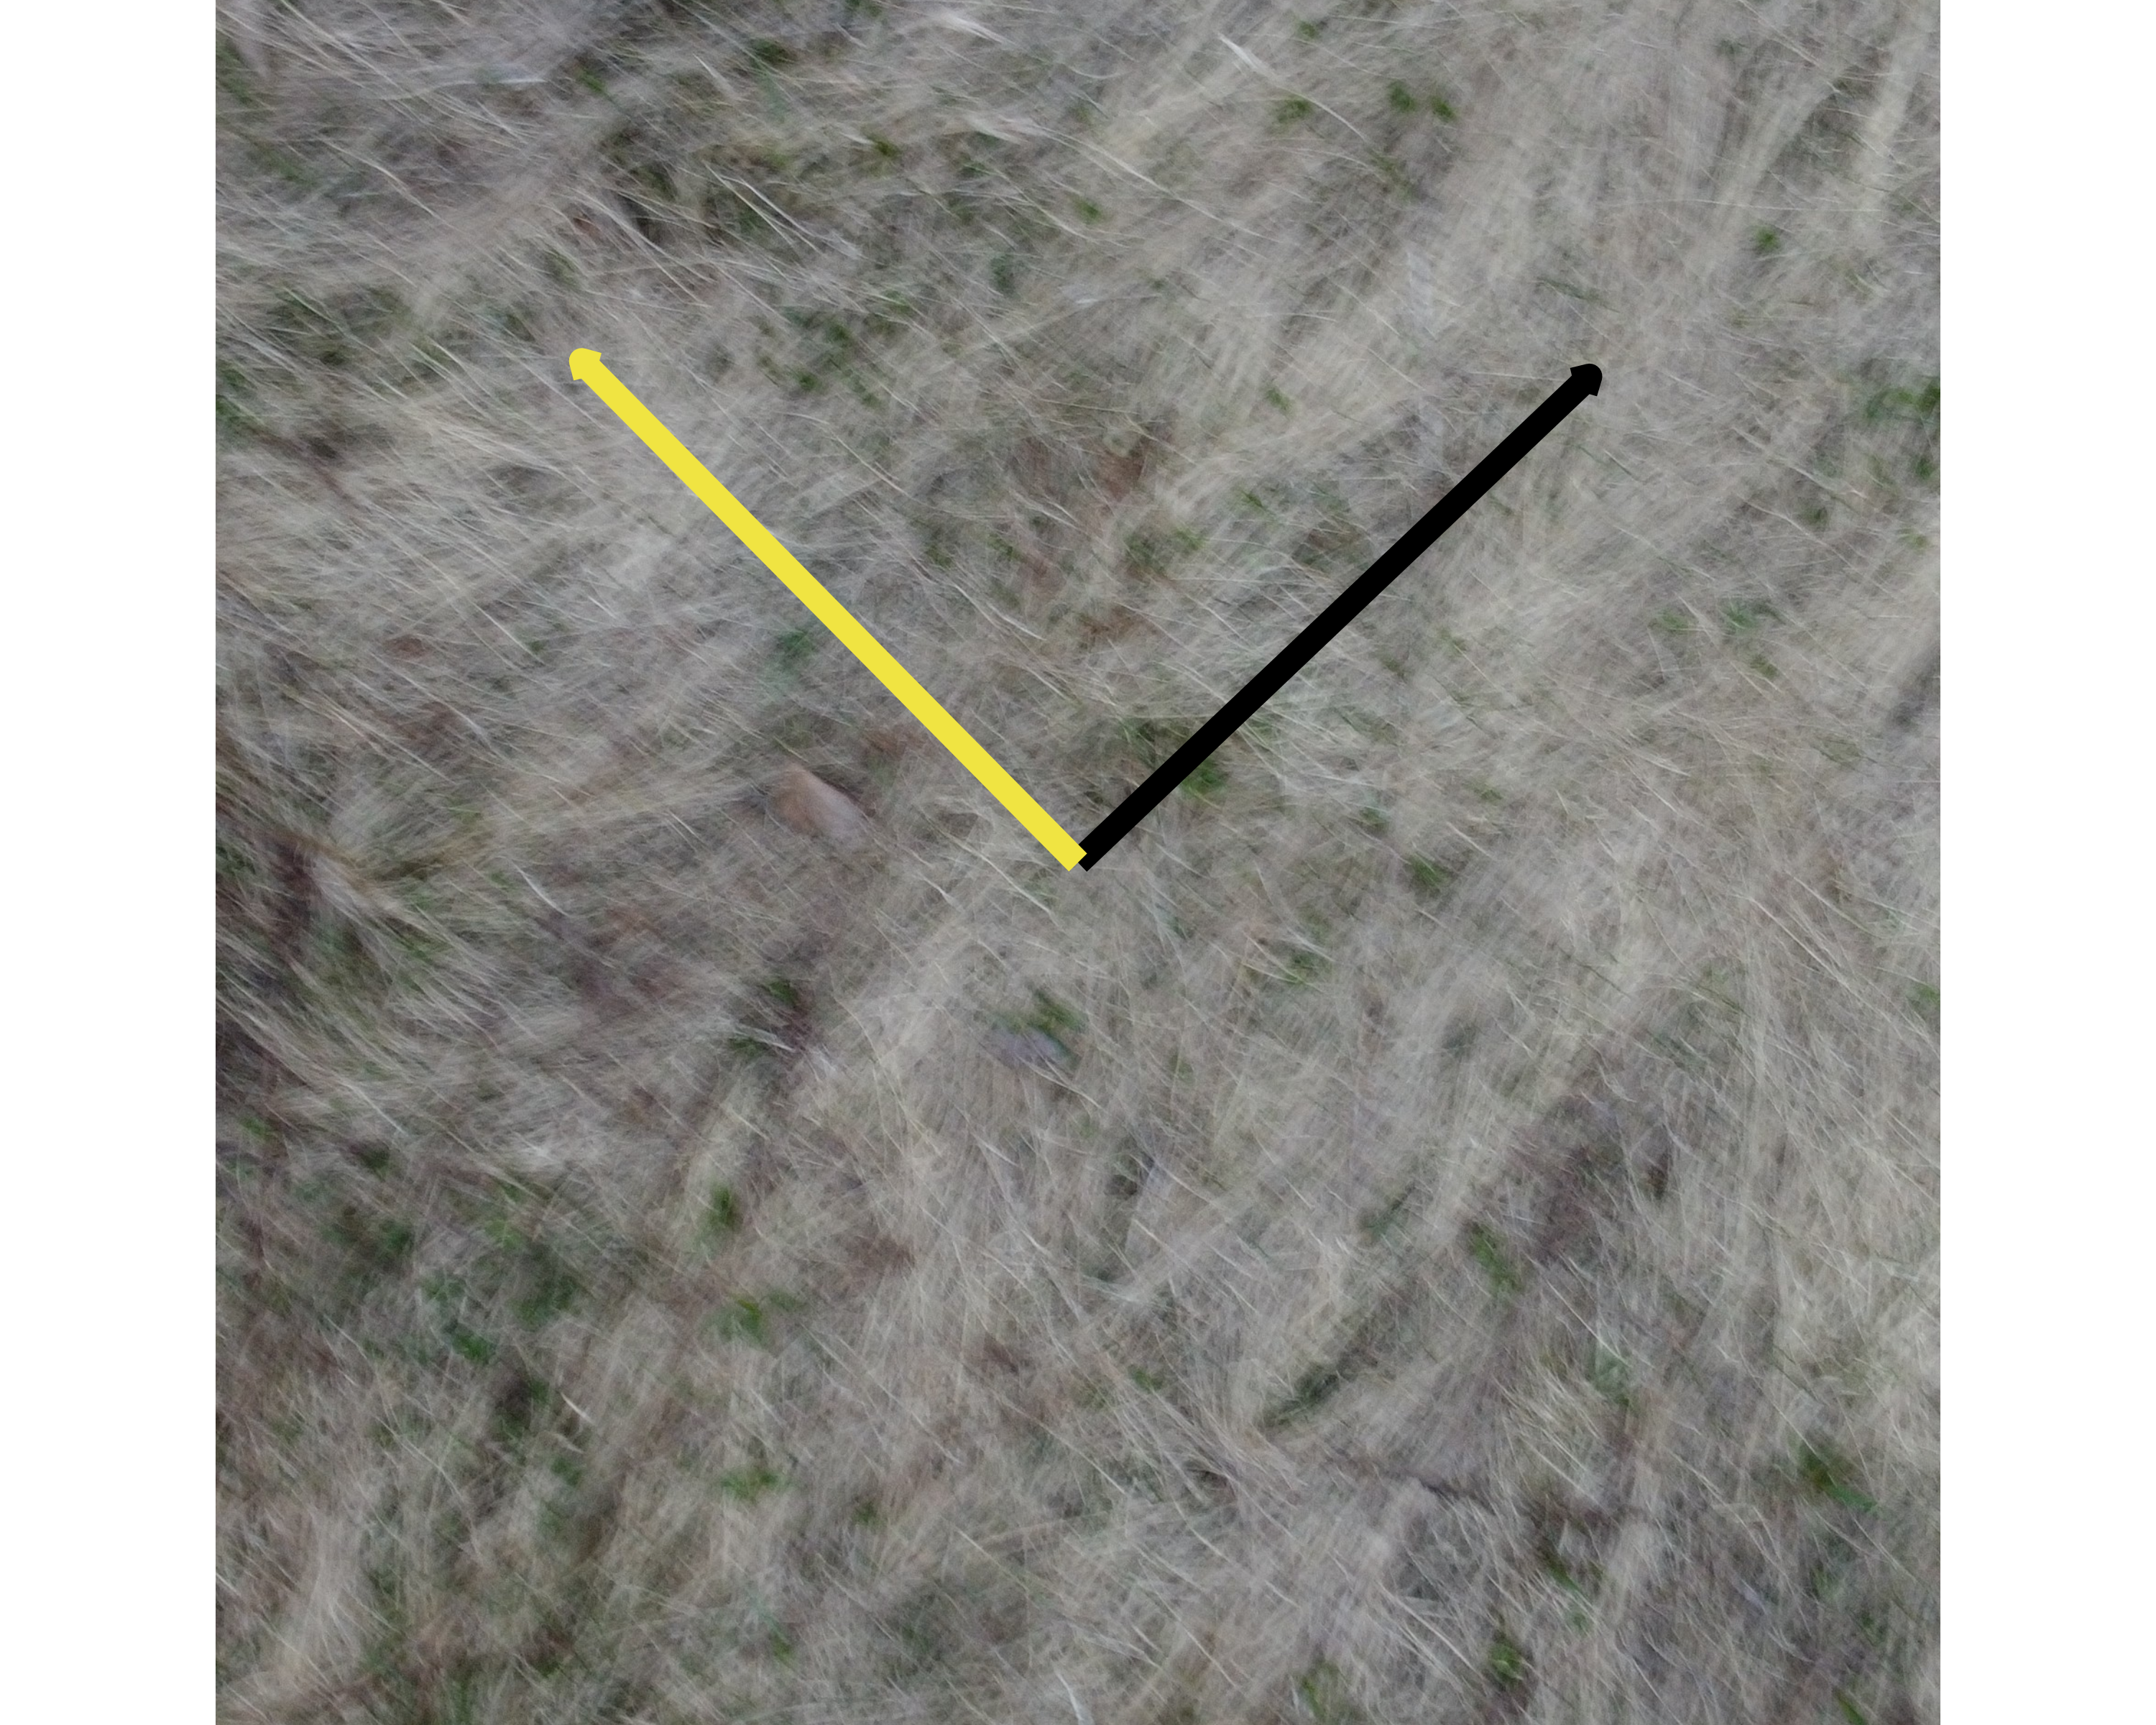
\includegraphics[width=0.8\linewidth,height=\textheight,keepaspectratio]{media/blurry_images.png}

}

\subcaption{\label{fig-resultblurry}High = 0.9999}

\end{minipage}%

\caption{\label{fig-results}Images Showing Circular Distance.}

\end{figure}%

There a number of reasons we assume the retrieved dominant angle differs
significantly between the gradient analysis and the human assessment.

The first is that while the gradient analysis uses magnitude weighting
in the circular statistics to give more influence to pixels with
stronger intensity changes, this weighting is applied across all pixels
in the image without first filtering out regions where no meaningful
grass structure exists. Pixels in flat, texturally uniform regions such
as bare soil, shadows, or background objects still produce gradient
responses, and even with low magnitudes they collectively contribute to
the overall dominant grass direction estimate. When many such
low-magnitude pixels are spread across non-grass regions of the image,
their cumulative effect can still shift the weighted circular mean away
from the true grass lay direction. A human observer instinctively
ignores these regions entirely, focusing attention only on areas where
grass texture is clearly visible. The algorithm, by contrast,
incorporates every pixel's contribution unless a magnitude threshold is
explicitly applied beforehand to exclude low-confidence regions, making
it more susceptible to being pulled by noise from non-grass areas of the
image.

A second source of disagreement is the variety of aerial perspectives
across the 65 images. Some images were captured from directly overhead,
providing a clear top-down view of grass lay patterns, while others were
taken at a lower angle closer to the grass surface, changing how
gradient directions are expressed in the image. Image quality like in
Figure~\ref{fig-resultblurry} produced blurry outlines and reduced
texture clarity. In such cases the gradient analysis struggles to
identify a coherent dominant direction, while human observers may still
be able to use contextual cues to make a reasonable directional
judgment.

\subsection{Comparing Dominant Grass Direction and Wind
Data}\label{comparing-dominant-grass-direction-and-wind-data}

At the SLU Living Lab, a wind station installed adjacent to the tundra
vegetation records wind speed and direction at 15-minute intervals via a
wind vane and anemometer as seen in Figure~\ref{fig-equipment}. To align
the wind data with the grass images, the 15-minute readings were
aggregated to daily circular mean wind directions using circular
statistics, accounting for the angular nature of wind direction data.
This produces one representative wind direction per day that captures
the overall prevailing direction across all readings that day.

To connect the grass images to the wind data, EXIF metadata that is the
Exchangeable Image File Format information embedded in every digital
image file was extracted from each drone image using the \texttt{exif}
package in R (Creative Computing Institute (2024)). The
\texttt{DateTimeOriginal} field was retrieved, which records the exact
date the image was captured by the drone, and cleaned into a
standardized date variable. Since the grass images were taken in April
2023, wind data from April through September 2022 (the full growing
season prior to image capture) was used for comparison. The rationale is
that grass lay direction observed in April 2023 reflects the cumulative
effect of winds experienced during the 2022 growing season when the
grass was actively growing and being shaped by prevailing conditions.

Nine representative images where the circular distance between gradient
analysis and human assessment was smallest were selected, representing
the cases where both methods most confidently agreed on a dominant grass
direction. The gradient analysis dominant direction for each of these
nine images was overlaid as a colored vertical line on polar histograms
of the monthly wind direction distributions from April through September
2022.

In Figure~\ref{fig-monthplots}, the grass lay directions from the nine
selected images are represented as colored vertical lines overlaid on
each month's wind direction polar histogram. The alignment between the
lines and the dominant bars of the wind histogram indicates months where
grass lay direction corresponds well with prevailing wind patterns. This
alignment is most evident in the spring months of April and May, which
represent the early growing season when grass is most actively
responding to wind exposure. This correspondence supports the use of
grass lay direction as a proxy for prevailing wind direction,
particularly during the growing season.

\begin{figure}[H]

\centering{

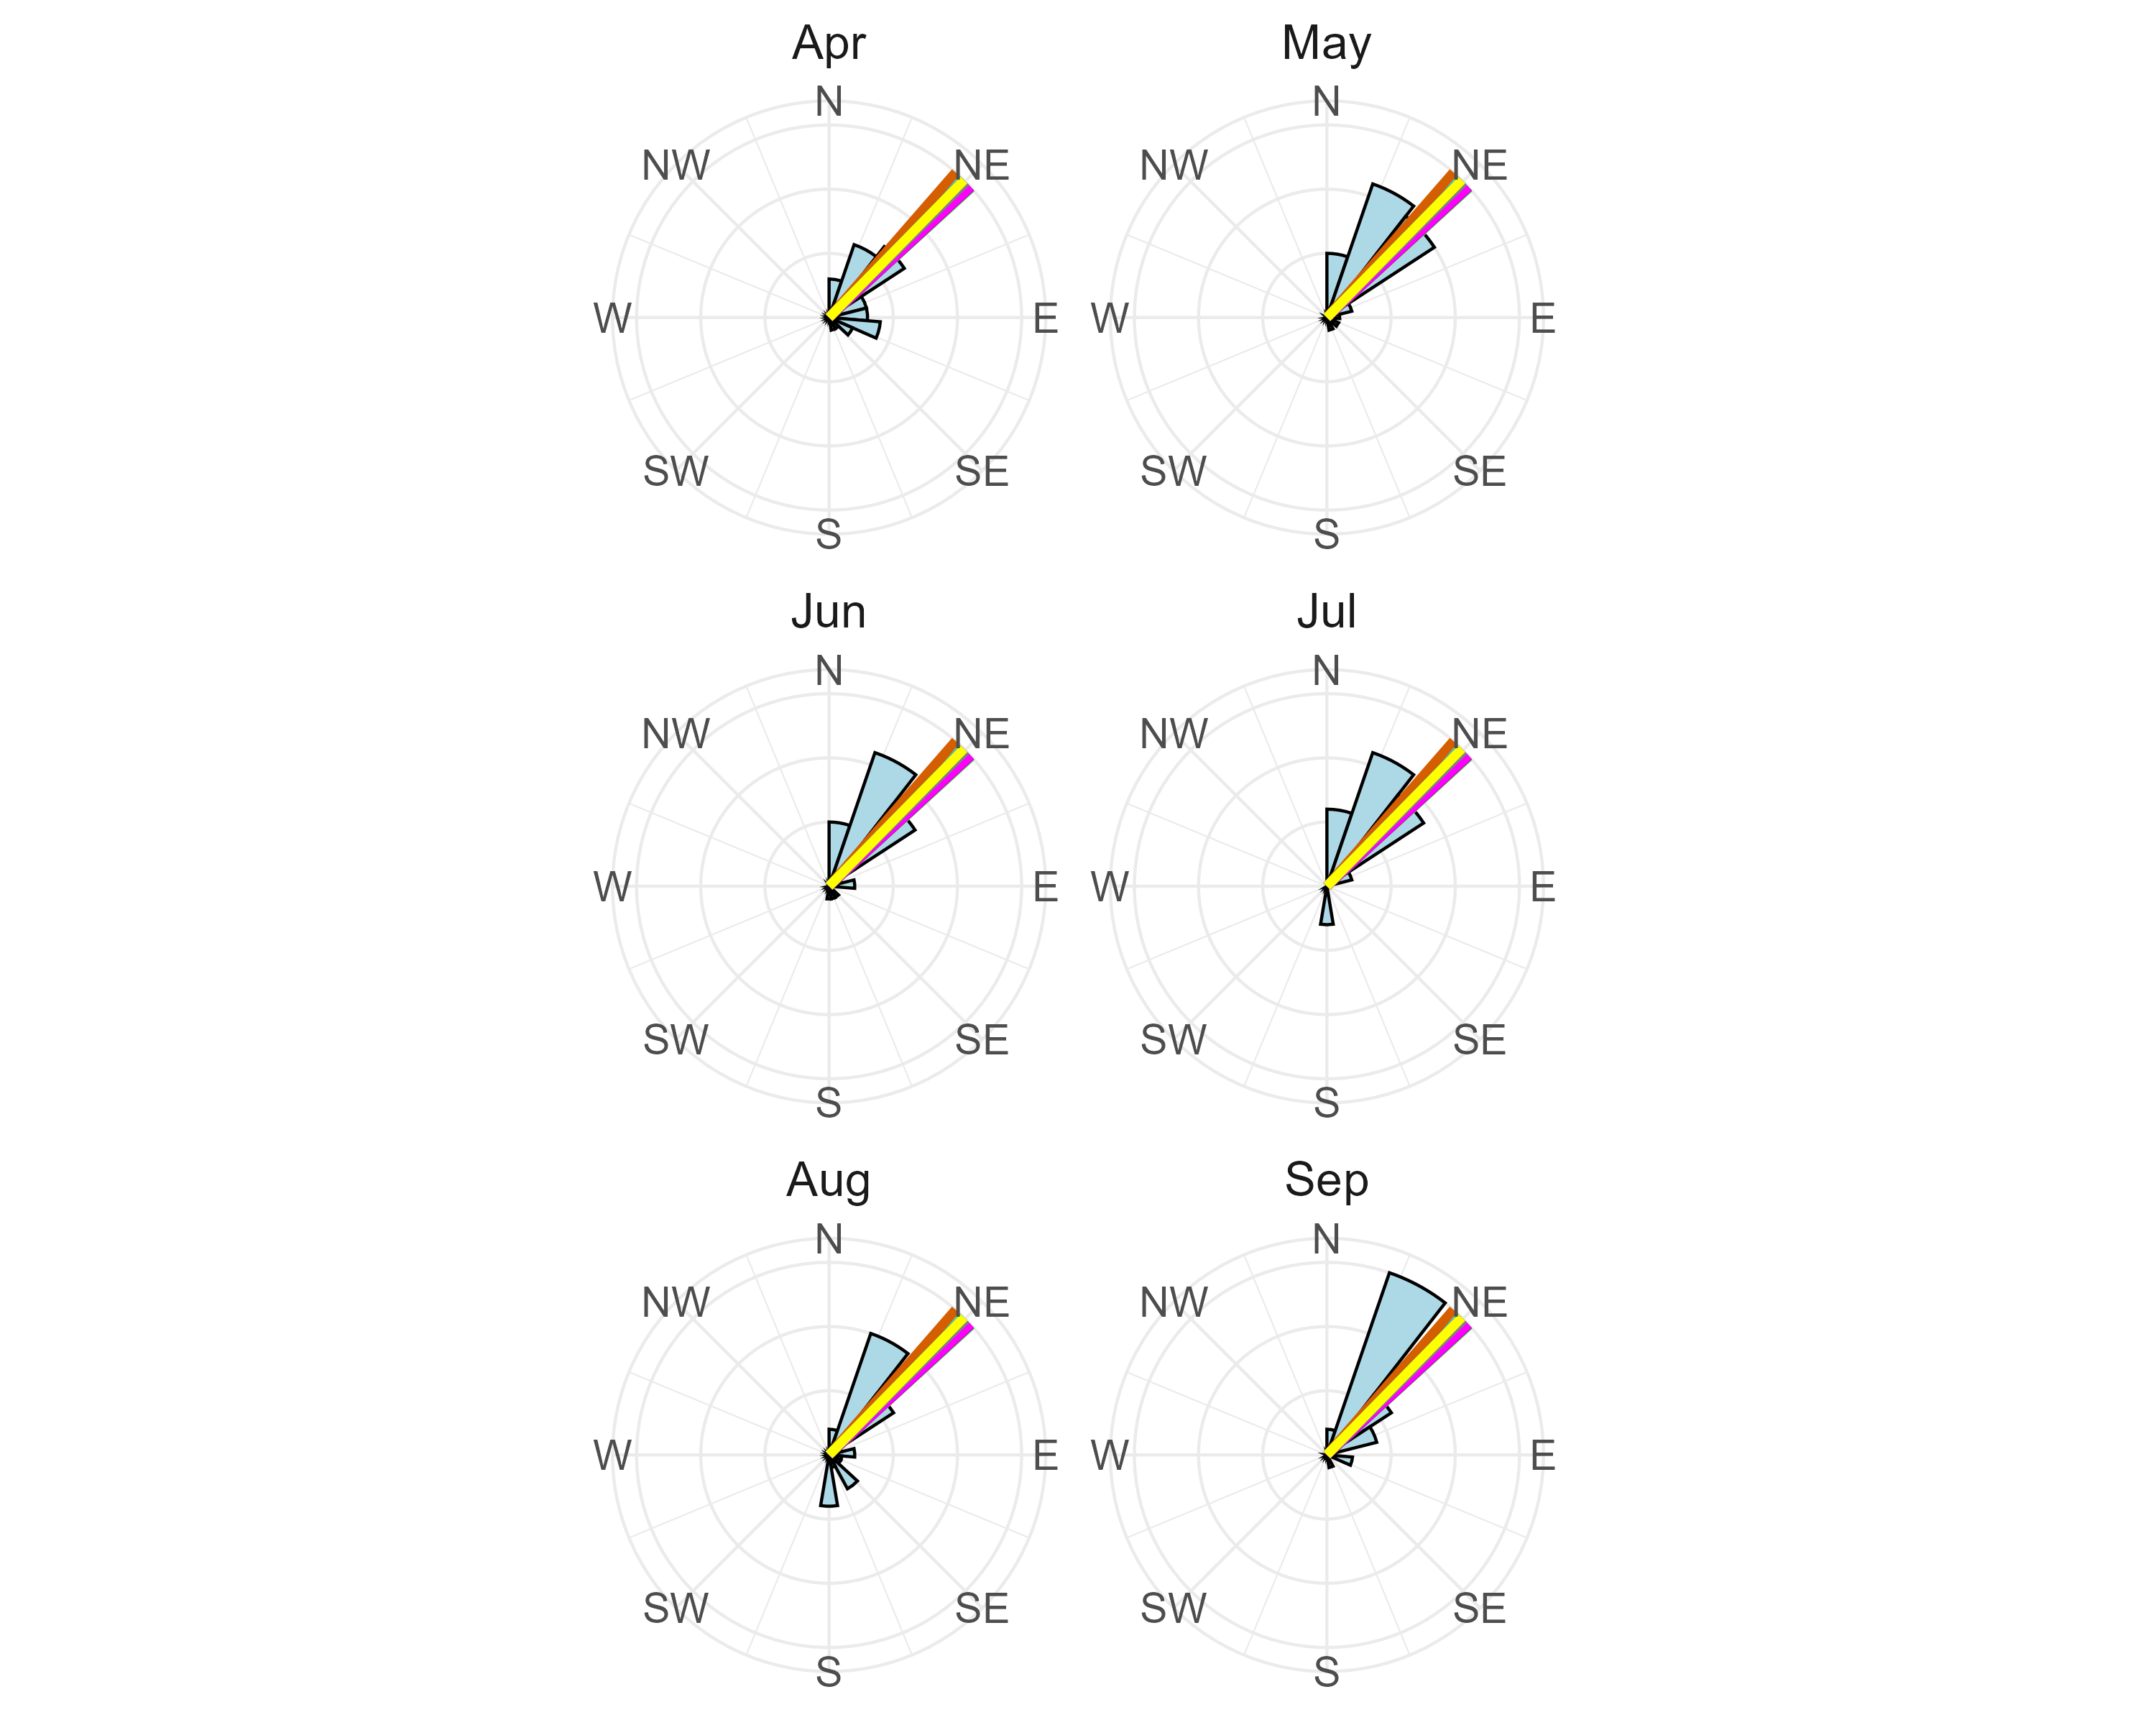
\includegraphics[width=1.2\linewidth,height=\textheight,keepaspectratio]{media/monthplots.png}

}

\caption{\label{fig-monthplots}Wind Data and Dominant Grass Lay From
Images.}

\end{figure}%

\clearpage

\section{Conclusion}\label{conclusion}

Overall, we find that in several images there is strong agreement
between human assessments and gradient-based estimates of dominant grass
direction. In these cases, both methods produce similar results,
suggesting that they can successfully capture the main direction of
grass lay from images. When compared with wind data, this alignment is
strongest in the spring season, which is the main growing period for
tundra grass. During this time, the grass is more flexible and
responsive to environmental conditions, making patterns of alignment
easier to detect.

However, there are still important cases where human assessments and
gradient-based methods do not agree, suggesting that both approaches may
have limitations. Human assessments can be affected by how clear or
complex the image is, while gradient methods can be influenced by image
noise, texture, or lighting conditions, and thus need algorithmic fine
tuning. Because of this, further work is needed to understand when each
method performs well and when it fails.

\subsection{Recommendations}\label{recommendations}

Based on the findings of this project, we offer the following
recommendations for future data collection, algorithmic improvement, and
community application.

\textbf{Image Collection Standards}

The results show that images taken at very high angles or with blurry
outlines consistently produced the highest circular distances between
gradient analysis and human assessment, indicating that image quality is
a significant driver of disagreement. We recommend that future drone
image collection for this purpose follow standardized protocols where
images should be taken directly overhead at a consistent altitude to
minimize perspective distortion, during daylight hours with minimal
shadow cover, and at a resolution sufficient to clearly resolve
individual grass blade texture. Standardizing these factors would reduce
variability in both human and computational assessments and improve the
reliability of comparisons across sites and seasons.

\textbf{Algorithmic Improvements}

The gradient analysis currently computes circular statistics across all
pixels in an image, including low-magnitude regions corresponding to
bare soil, shadows, and background objects that carry no meaningful
grass orientation signal. Even with magnitude weighting, the cumulative
contribution of these regions can shift the dominant direction estimate.
We recommend applying an explicit magnitude threshold filter before
computing circular statistics to retain only pixels with gradient
magnitudes above a meaningful level. Fine-tuning an optimal threshold
that is potentially image-specific and based on the magnitude
distribution would be a valuable next step toward improving the
algorithm's accuracy.

\textbf{Human vs.~Automated Assessment}

There is also potential for practical application beyond research. A
simple web-based tool could allow community members or local observers
to upload field images and estimate local wind direction automatically.
The choice between human crowd-sourcing and automated gradient analysis
likely depends on the goal and context of use. In communities like
Savoonga where TEK already involves the practice of physically observing
grass lay, expanding human participation through crowd-sourcing may be
the more natural and culturally appropriate approach where more
observers following the same traditional practice would help
standardize, recalibrate, and strengthen the existing knowledge system
rather than replacing it. In contrast, for research contexts where
eliminating human perceptual bias and subjectivity is important, or
where large volumes of images need to be processed consistently across
sites, the gradient analysis offers a more scalable and repeatable
alternative. The best approach therefore depends not just on image
quality or algorithmic performance, but on whether the goal is to
support and scale an existing human observational practice or to provide
an objective computational tool independent of human judgment.

\subsection{Future Work}\label{future-work}

These results have shown promising agreement between human perception,
computational methods, and wind data in certain conditions. At the same
time, they highlight the importance of improving data collection
practices, understanding sources of disagreement, and expanding
fine-tuning goals. Future analysis should focus on disagreement cases in
more detail to identify when vegetation direction is not a reliable
indicator of wind, or when one method is more accurate than the other.
It would also be useful to compare results across different years, such
as using 2023 wind data and 2024 grass images, to test whether these
patterns remain consistent over time and under different environmental
conditions. This project could also be expanded beyond tundra grass to
other vegetation types that respond to wind in different seasons.
Together, these steps move toward a more robust framework for linking
image-based vegetation analysis with environmental wind patterns in
support of both scientific understanding and Traditional Ecological
Knowledge.

\clearpage

\section*{References}\label{references}
\addcontentsline{toc}{section}{References}

\protect\phantomsection\label{refs}
\begin{CSLReferences}{1}{1}
\bibitem[\citeproctext]{ref-cci2024}
Creative Computing Institute. 2024. \emph{Intro to EXIF Image Metadata}.
\url{https://wiki.cci.arts.ac.uk/books/how-to-guides/page/intro-to-exif-image-metadata}.

\bibitem[\citeproctext]{ref-indigenous2013}
Huntington, Henry P., Nicole M. Braem, Caroline L. Brown, et al. 2013.
{``Local and Traditional Knowledge Regarding the Bering Sea Ecosystem:
Selected Results from Five Indigenous Communities.''} \emph{Science
Direct} 94: 322--34.

\bibitem[\citeproctext]{ref-kawerak2024savoonga}
Kawerak Inc. 2024. \emph{Savoonga}.
\url{https://kawerak.org/our-region/savoonga/}.

\bibitem[\citeproctext]{ref-manavalan2020}
Manavalan, R. 2020. {``Automatic Identification of Diseases in Grains
Crops Through Computational Approaches: A Review.''} \emph{Science
Direct} 178: 8--10.

\bibitem[\citeproctext]{ref-definetek}
Oregon State University Traditional Ecological Knowledge Lab. 2026.
{``What Is TEK?''} \url{https://tek.forestry.oregonstate.edu/what-tek}.

\bibitem[\citeproctext]{ref-defineplotly}
Plotly Technologies Inc. 2026. {``Plotly r Graphing Library.''}
\url{https://plotly.com/r/}.

\bibitem[\citeproctext]{ref-defineshiny}
Posit. 2026. {``Welcome to Shiny.''}
\url{https://shiny.posit.co/r/getstarted/shiny-basics/lesson1/}.

\bibitem[\citeproctext]{ref-rosales2021}
Rosales, Jon, Ivan Ramler, Lisa Torrey, Aaron Iverson, and Perry
Pungowiyi. 2021. \emph{Measuring Wind Direction Change on {St. Lawrence
Island, Alaska} with Traditional Ecological Knowledge}. NSF Arctic
Social Science Solicitation, Award No. 21-526.

\bibitem[\citeproctext]{ref-slulivinglab}
St. Lawrence University. 2026b. {``Living Lab.''}
\url{https://sites.stlawu.edu/livinglab/}.

\bibitem[\citeproctext]{ref-slulab}
St. Lawrence University. 2026a. {``Living Lab.''}
\url{https://www.stlawu.edu/offices/environmental-studies/living-lab}.

\bibitem[\citeproctext]{ref-sunshine2024}
Sunshine, Ben. 2024. {``Applying the Histogram of Oriented Gradients
Algorithm for Detecting Grass Lay Direction.''} Unpublished manuscript.

\end{CSLReferences}




\end{document}
